\documentclass[10pt]{article}
\usepackage{iftex}

\usepackage[hmargin=2.2cm, vmargin=2cm]{geometry}
\usepackage{frenchmath}
\usepackage[dvipsnames,table]{xcolor}
\usepackage{colortbl}
\usepackage{fontspec}
\usepackage{tabularx}
\usepackage{tikz}
\usetikzlibrary{patterns}
\usetikzlibrary{calc}
\usetikzlibrary{math}
\usepackage{amsmath}
\usepackage{scratch3}
\usepackage{wrapfig}

\usepackage[locale=FR, group-digits=all, group-separator=\ , group-minimum-digits=4]{siunitx}
\DeclareSIUnit{\cube}{\cubed}
\DeclareSIUnit{\carre}{\squared}
\DeclareSIUnit{\litre}{\ell}
\usepackage{eurosym}
\DeclareSIUnit{\EURO}{\text{\footnotesize{\euro}}}

\definecolor{Carmin}{HTML}{C61932}
\setlength{\parindent}{0pt}

\setsansfont{Archive}[
    Path=../../Polices/Archive/,
    Extension = .otf,
    UprightFont=*
    ]
    
\setromanfont{Marianne}[
    Path=../../Polices/Marianne/,
    Scale=0.8,
    Extension = .otf,
    UprightFont=*-Regular,
    BoldFont=*-Bold,
    ItalicFont=*-RegularItalic,
    BoldItalicFont=*-BoldItalic
    ]
    
\DeclareMathSizes{10}{8}{7}{7} % Pour ajuster la taille des mathématiques et du reste du texte

\pagestyle{empty}
\rmfamily

% Titre du document
\newcommand{\titre}{\sffamily{\huge\color{Carmin}\centerline{ATTENDUS DE FIN D'ANNÉE DE 6\textsuperscript{E}}}\rmfamily}


% Trois symboles
\newcommand{\RR}{
\begin{tikzpicture} \draw[Carmin,fill=Carmin] (0,0) circle (0.06); \end{tikzpicture}}
\newcommand{\LR}{\begin{tikzpicture} \draw[Carmin,fill=Carmin] (0.05,0) -- (0,0.075) -- (-0.05,0) -- (0,-0.075) --cycle; \end{tikzpicture}}
\newcommand{\CR}{\begin{tikzpicture} \draw[Carmin,fill=Carmin] (0,0) -- (0,0.1) -- (0.1,0.1) -- (0.1,0) -- cycle; \end{tikzpicture}}

% Thèmes
\newcommand{\theme}[1]
{\vspace{4ex}\begin{tabularx}{\textwidth}{|XXXX|}\arrayrulecolor{Carmin}
    \multicolumn{4}{c}{\sffamily\color{white}\cellcolor{Carmin}\Large{\phantom{É}#1\phantom{É}}\rmfamily} \\\normalsize
    \RR{} Ce que sait faire l'élève & \LR{} Type d'exercice & \CR{} Exemple d'énoncé & \textit{Indication générale} \\\hline
\end{tabularx}\vspace{3ex}}

% Compétences
\newcommand{\competence}[1]{\par\color{Carmin}\makebox[\linewidth]{\rule{\textwidth}{2pt}}\\{\bfseries\Large#1}\color{black}\vspace{1em}}
\newcommand{\souscompetence}[1]{\par\color{Carmin}\textbf{\large{#1}}\color{black}\vspace{1em}}

% Liste "ce que sait faire l'élève"
\newenvironment{savoireleves}{%
    \renewcommand{\labelitemi}{\RR}%
    \color{black}%
    \par\textbf{Ce que sait faire l'élève}
    \begin{itemize}
    \setlength{\itemsep}{-0.2em}%
}{
    \end{itemize}
}

% Liste "exemples de réussite"
\newenvironment{exemplesreussite}{%
    \renewcommand{\labelitemi}{\LR}%
    \renewcommand{\labelitemii}{-}%
    \color{black}%
    \par\textbf{Exemples de réussite}
    \begin{itemize}
    \setlength{\itemsep}{-0.2em}%
}{
    \end{itemize}
}

\newenvironment{sousitemize}{
    \color{black}%
    \vspace{-1em}%
    \begin{itemize}
    \setlength{\itemsep}{0em}%
}{
    \end{itemize}
}

\newenvironment{sousenumerate}{
    \color{black}%
    \vspace{-1em}%s
    \begin{enumerate}
    \setlength{\itemsep}{0em}%
}{
    \end{enumerate}
}


%%%%%%%%%%%%%%%%%%%%%%%%%%%%%%%%%%%%%%%%%%%%%%%%%%%%%%%%%%%%%%%%%%
%%%%%%%%%%%%%%%%%%%%%%%%%%%%%%%%%%%%%%%%%%%%%%%%%%%%%%%%%%%%%%%%%%
%%%%%%%%%%%%%%%%%%%%%%%%%%%%%%%%%%%%%%%%%%%%%%%%%%%%%%%%%%%%%%%%%%

\begin{document}
    \titre
    \theme{NOMBRES ET CALCULS}
    \competence{Utiliser et représenter les grands nombres entiers, des fractions simples, les nombres décimaux}

    \begin{savoireleves}
        \item Il sait utiliser les grands nombres entiers.
        \item Il utilise des nombres décimaux ayant au plus quatre décimales.
        \item Il sait faire le lien entre « la moitié de » et multiplier par $\frac{1}{2}$.
        \item Il ajoute des fractions décimales de même dénominateur.
        \item Il ajoute des fractions de même dénominateur.
        \item Il sait utiliser des fractions pour exprimer un quotient. Il comprend que $\frac{a}{b} \times b = a$.
        \item Il sait utiliser des fractions pour rendre compte de mesures de grandeurs.
    \end{savoireleves}
    
    \begin{exemplesreussite}
        \item Il écrit en chiffres dix-sept milliards vingt-trois millions quatre cent cinq.
        \item Il recopie la phrase suivante en écrivant le nombre en chiffres : « Au mois de juin 2018, la population mondiale est d’environ sept milliards cinq cent cinquante-neuf millions deux cent quatre-vingt-huit mille trois cents personnes. »
        
        \item[\CR] Complète l’égalité : 3 dizaines de milliards et 8 millions = … millions.
        \item[\CR] Voici cinq cartes contenant un nombre : \boxed{415}  \boxed{2103}  \boxed{9}  \boxed{87}  \boxed{13}.
        Place ces cartes côte à côte pour écrire :
        \begin{sousitemize}
            \item le plus petit nombre entier faisable de douze chiffres
            \item le plus grand nombre entier faisable de douze chiffres
        \end{sousitemize}
        \item Jeu du nombre mystère (avec des millions) écrit derrière le tableau par le professeur. L’élève, tout seul ou dans un groupe, le retrouve en ne posant que des questions du type : « Est-il plus petit que... ? » ou « Est-il plus grand que... ? »
        \item Sans utiliser le mot « virgule », il lit et écrit de différentes façons le nombre 15,3062 :
        \begin{sousitemize}
            \item 15 unités et 3 062 dix-millièmes
            \item 153 062 dix-millièmes
            \item $(1 \times 10) + (5 \times 1) + \frac{3}{10} + \frac{6}{1000} + \frac{2}{10000}$
            \item $15 + \frac{3062}{10000}$
        \end{sousitemize}

        \item À partir des renseignements qui suivent, il trouve le nombre caché : (Réponse : 2,5842)
        \begin{sousenumerate}
            \item C’est un nombre décimal de 5 chiffres.
            \item Son chiffre des dixièmes est le même que celui de 17,54.
            \item Son chiffre des centièmes est le chiffre des unités de millions de 738 214 006.
            \item Son chiffre des unités est le chiffre des dizaines de mille de 120 008.
            \item Son chiffre des millièmes est la moitié de celui des centièmes.
            \item Son chiffre des dix-millièmes est égal au chiffre des unités.
        \end{sousenumerate}
        \item Il range dans l’ordre croissant les six nombres suivants écrits de différentes façons :
        \begin{sousitemize}
            \item $\frac{6}{10} + \frac{1}{100} + \frac{1}{10000}$
            \item six cent onze millièmes
            \item $6,1111$
            \item $6+\frac{101}{1000}$
            \item $6111$ dix-millièmes
            \item $\frac{6101}{10000}$
        \end{sousitemize}
        \clearpage
        \item Il identifie combien de nombres différents sont écrits dans la liste ci-dessous : 
        \begin{sousitemize}
            \item $\frac{1284}{10000}$
            \item $\frac{1}{4}$
            \item $0,25$
            \item $1,4$
            \item $\frac{25}{100}$
        \end{sousitemize}
        
        \item Il écrit le nombre qui correspond au point A : 
        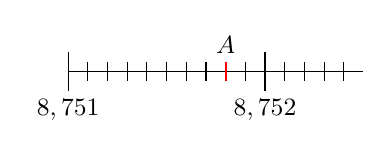
\begin{tikzpicture}[scale=0.25]
            \draw (0,0) -- (15,0);
            \foreach \x in {0,1,...,14} {
                \draw (\x,0.5) -- (\x,-0.5);
            }
            \draw (0,1) -- (0,-1);
            \draw (10,1) -- (10,-1);
            \draw[thick,red] (8,0.5) -- (8,-0.5);
            \node[above] at (8,0.4) {\small{$A$}};
            \node[below] at (0,-0.9) {\small{$8,751$}};
            \node[below] at (10,-0.9) {\small{$8,752$}};
        \end{tikzpicture}
        
        \item Il écrit le nombre qui convient dans le rectangle :
        
        \begin{tikzpicture}[scale=0.4]
            \draw[-latex] (0,0) -- (18.5,0);
            \foreach \x in {2,...,17} {
                \draw (\x,0.5) -- (\x,-0.5);
            }
            \draw (1.5,-3) -- (11.5,-3);
            \foreach \x in {2.5,3.5,...,10.5} {
                \draw (\x,-2.5) -- (\x,-3.5);
            }
            \draw (4.5,-6) -- (14.5,-6);
            \foreach \x in {5.5,6.5, ...,13.5} {
                \draw (\x,-6.5) -- (\x,-5.5);
            }
            \draw (3,-9) -- (13,-9);
            \foreach \x in {4,5,...,12} {
                \draw (\x,-8.5) -- (\x,-9.5);
            }
            % Grandes graduations
            \node at (4,1.3) {\small{300}};
            \node at (14,1.3) {\small{400}};
            \draw (4,1) -- (4,-1);
            \draw (14,1) -- (14,-1);
            \draw (1.5,-2) -- (1.5,-4);
            \draw (11.5,-2) -- (11.5,-4);
            \draw (4.5,-5) -- (4.5,-7);
            \draw (14.5,-5) -- (14.5,-7);
            \draw (3,-8) -- (3,-10);
            \draw (13,-8) -- (13,-10);
            % Reliures entre les segments
            \draw[densely dotted] (7,-0.5) -- (1.5,-2) (8,-0.5) -- (11.5,-2);
            \draw[densely dotted] (11.5,-4) -- (14.5,-5) (10.5,-3.5) -- (4.5,-5);
            \draw[densely dotted] (5.5,-6.5) -- (3,-8) (6.5,-6.5) -- (13,-8);
            % Le rectangle
            \draw[-stealth] (9,-11) -- (9,-9.7);
            \draw (8,-12) rectangle (10,-11.1);
        \end{tikzpicture}
        
        \item Il intercale un nombre décimal entre 3,451 et 3,452.
        \item Il encadre le nombre 28,4597 :
        \begin{sousitemize}
            \item par deux nombres entiers consécutifs
            \item par deux nombres décimaux, au dixième près
            \item par deux nombres décimaux, au centième près
            \item puis, par deux nombres décimaux, au millième près.
        \end{sousitemize}

        \item Il calcule et fait le lien entre : 
        \begin{sousitemize}
            \item la moitié de 28
            \item $28 \times \frac{1}{2}$
            \item $50~\%$ de 28
        \end{sousitemize}
        Il pourra ensuite calculer $28 \times 1,5$ en utilisant le fait que $1,5 = 1 + \frac{1}{2}$.
        \item Il calcule et fait le lien entre le quart de $80$, $\frac{1}{4}$ de $80$ et $25~\%$ de $80$.
        \item[\CR] Calcule $\frac{3}{10}+\frac{4}{10}$ ; $\frac{26}{100}+\frac{31}{100}+\frac{43}{100}$ ; $\frac{7}{10}+\frac{3}{10}$.
        \item[\CR] Calcule $\frac{3}{5} + \frac{4}{5}$ ; $\frac{26}{25} + \frac{31}{25} + \frac{43}{25}$ ; $\frac{7}{2}+\frac{3}{2}$. 
        \item Il verbalise que sept fois deux septièmes c’est deux, que le septième de deux, c’est deux septièmes et que deux fois un septième c’est deux septièmes.
        \item Il calcule : $\frac{2}{7} \times 7$ ; $\frac{31}{51} \times 51$
        \item[\CR] Complète les égalités suivantes : \[ 4 \times ... = 8 ~~~~~~ 4 \times ... = 10 ~~~~~~ 4 \times ... = 11 \]
        \item Il exprime la largeur exacte d’un rectangle de longueur \qty{7}{\centi\metre} et d’aire \qty{23}{\centi\metre\carre}. Il encadre la mesure trouvée par deux nombres entiers consécutifs de centimètres.
    \end{exemplesreussite}
    
    \clearpage
    \competence{Calculer avec des nombres entiers et des nombres décimaux}
    
    \begin{savoireleves}
        \item[] \textbf{\textit{Calcul mental ou en ligne}}
        \item Il sait multiplier un nombre décimal (entier ou non) par $0,1$ et par $0,5$.
        \item Il sait utiliser la distributivité simple dans les deux sens.
        \item Il apprend à organiser un calcul en une seule ligne, utilisant si nécessaire des parenthèses.
        \item[] \textbf{\textit{Calcul instrumenté}}
        \item Il sait utiliser une calculatrice pour introduire la priorité de la multiplication sur l’addition et la soustraction.
        \item[] \textbf{\textit{Calcul posé}}
        \item Il sait multiplier deux nombres décimaux.
    \end{savoireleves}
    
    \begin{exemplesreussite}
        \item[] \textbf{\textit{Calcul mental ou en ligne}}
        \item Il calcule :
        \begin{sousitemize}
            \item[] $5,8792 \times 10$ (en lien avec la numération : la valeur de chaque chiffre devient 10 fois plus grande : 5 unités $\times 10 =$ 5 dizaines, 8 dixièmes $\times 10 = 8$ unités...) 
            \item[] $45 621 \div 10 000$ (en lien avec la numération : la valeur de chaque chiffre devient 10 000 fois plus petite : 1 unité $\div 10000 = 1$ dix-millième)
        \end{sousitemize}

        \item Il calcule $25 \times 3,5679 \times 4$ en regroupant $(25 \times 4) \times 3,5679$.
        \item Il calcule $0,6 \times 0,4$ ou encore $22 \times 0,5$.
        \item Il calcule $780 \times 0,1$ en utilisant $780 \times 1~\text{dixième} = 780~\text{dixièmes} = 78$. Il fait le lien avec $780 \div 10$.
        \item Il calcule $3,5 \times 0,001$ en utilisant les règles de la multiplication ou en faisant le lien avec la division par $1 000$.
        \item Il calcule 
        \begin{sousitemize}
            \item $13 \times 7 + 13 \times 3$ en passant par $13 \times 10$
            \item $32 \times 11$ en décomposant $32 \times 10 + 32 \times 1$
            \item $32 \times 19$ en décomposant $(32 \times 2 \times 10) - (32 \times 1)$, en utilisant le fait que $19 = 20 - 1$.
        \end{sousitemize}
        \item Il sait trouver un ordre de grandeur de $9,8 \times 24,85$ en calculant par exemple $10 \times 25$.
        \item En utilisant ses connaissances sur le produit de deux décimaux et un ordre de grandeur, il sait trouver la réponse exacte du calcul $9,52 \times 51,3$ parmi les réponses proposées : \boxed{488,76} \boxed{48,376} \boxed{488,375} \boxed{488,376} \boxed{488 376}.
        \item Il est capable d'écrire puis de calculer $\qty{7,50}{\EURO} + (3 \times \qty{4,90}{\EURO})$.
        \item[\CR] Calcule le périmètre du rectangle ci-dessous :
        
        \begin{center}
        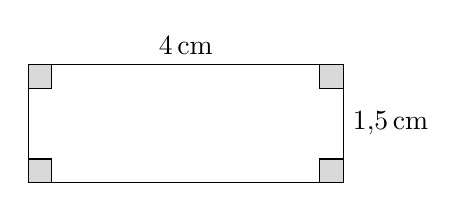
\begin{tikzpicture}
            \draw (0,0) rectangle (4,1.5);
            \draw[fill=gray!30!white] (0,0) rectangle (0.3,0.3) (4,0) rectangle (3.7,0.3) (0,1.5) rectangle (0.3,1.2) (4,1.5) rectangle (3.7,1.2);
            \node[above] at (2,1.5) {\qty{4}{\centi\metre}};
            \node[anchor=west] at (4,0.75) {\qty{1.5}{\centi\metre}};
        \end{tikzpicture}
        \end{center}
        
        \textit{Il écrit puis calcule :}\\
        $2 \times \qty{4}{\centi\metre} + 2 \times \qty{1.5}{\centi\metre} = 2 \times (\qty{4}{\centi\metre} + \qty{1.5}{\centi\metre}) = 2 \times \qty{5.5}{\centi\metre} = \qty{11}{\centi\metre}$
        \item[\CR] Paolo achète dans un magasin un DVD à \qty{7.50}{\EURO} et trois CD à \qty{4.90}{\EURO} l'unité. Combien va-t-il payer ?
        \item[] \textbf{\textit{Calcul instrumenté}}
        \item Arthur calcule mentalement $3 + 4 \times 8$ et trouve $35$. Alice utilise une calculatrice et trouve $56$. L’élève sait expliquer d’où vient cette différence.
        \item[] \textbf{\textit{Calcul posé}}
        \item Il sait poser et effectuer le produit $18,56 \times 7,9$.
    \end{exemplesreussite}
    
    \clearpage
    \competence{Résoudre des problèmes en utilisant des fractions simples, les nombres décimaux et le calcul}
    
    \begin{savoireleves}
        \item Il résout des problèmes relevant des structures additives et multiplicatives en mobilisant une ou plusieurs étapes de raisonnement.
        \item Il collecte les informations utiles à la résolution d'un problème à partir de supports variés, les exploite et les organise en produisant des tableaux à double entrée, des diagrammes circulaires, semi-circulaires, en bâtons ou des graphiques.
        \item Il remobilise les procédures déjà étudiées pour résoudre des problèmes relevant de la proportionnalité et les enrichit par l'utilisation du coefficient de proportionnalité.
        \item Il sait appliquer un pourcentage.
    \end{savoireleves}
    
    \begin{exemplesreussite}
        \item[\CR] Sachant que $685 \times 26 = 17 810$, résous chacun des problèmes suivants :
        \begin{sousitemize}
            \item[\CR] Le CDI achète $26$ revues à \qty{6,85}{\EURO} l’une. Combien vont coûter les revues ?
            \item[\CR] Hier, Monsieur Truc, apiculteur, a rempli $26$ pots de miel de \qty{685}{\g} chacun. Quelle quantité totale de miel l’apiculteur a-t-il mise en pots hier ?
            \item[\CR] Élisa achète \qty{2,6}{\kg} de fraises à \qty{6.85}{\EURO} le kg. Combien va-t-elle payer les fraises ?
        \end{sousitemize}
        \item[\CR] En $2018$, la Chine comptait un-milliard-trois-cent-quatre-vingt-quinze-millions-deux-cent-trois-mille-quatre-cents habitants. C'est trente-neuf-millions-cinq-cent-quatre-vingt-un-mille-six-cent de plus qu'en Inde. Combien y-a-t-il d'habitants \raggedright{en Inde ?}
        \item[\CR] J'achète \qty{1.6}{\kg} de bananes qui coûtent $3,25$ euros le kg. Je dispose d’un billet de $5$ euros. Ai-je assez d'argent ?
        \item[\CR] Un initiateur de tennis achète sur internet $16$ raquettes à \qty{8.50}{\EURO} l’unité et $20$ cerceaux. Il paye au total \qty{192}{\EURO}. Quel est le prix d'un cerceau ?
        \item[\CR] En $5$ jours, le pirate Long John Silver a déposé $135$ pièces d'or dans son coffre. Chaque jour, il a déposé sept pièces d'or de plus que le jour précédent. Combien de pièces d'or avait-il déposé le premier jour ?
        \item[\CR] Je suis un multiple de $7$ compris entre $40$ et $100$ dont la somme des chiffres est un multiple de $4$. Qui suis-je ?
        \item[\CR] Dans un collège, les enfants ont le choix d'étudier $3$ langues pour la langue vivante $2$ : italien, allemand ou espagnol.\\
            En 5e A, il y a $25$ élèves. $12$ ont choisi espagnol, $6$ allemand et les autres italien.\\
            En 5e B, $13$ élèves ont choisi espagnol et $5$ élèves allemand.\\
            Dans ces deux classes, $12$ élèves ont choisi italien.\\
            Présenter ces données dans un tableau à double entrée.
        \item[\CR] Dis si l'affirmation suivante est vraie ou fausse à partir du graphique ci-dessous :
        
        \begin{center}
        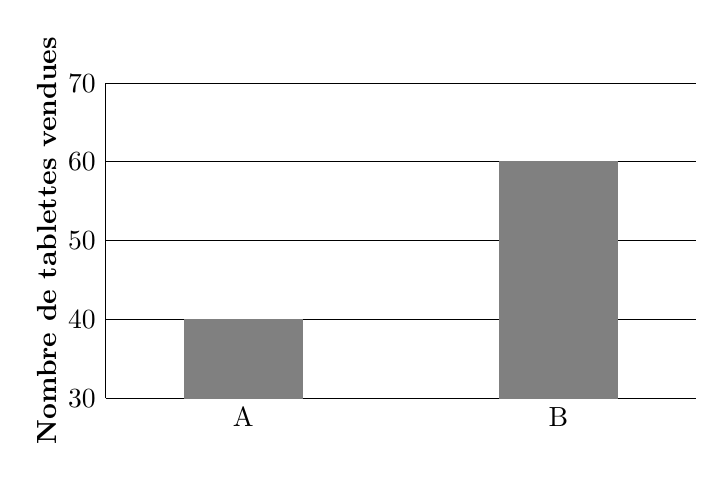
\begin{tikzpicture}[scale=0.5]
            \foreach \y/\valeur in {0/30,2/40,4/50,6/60,8/70} {
                \draw (0,\y) -- (15,\y);
                \node[anchor=east] at (0,\y) {\valeur};
            }
            \draw (0,0) -- (0,8);
            \draw[gray,fill=gray] (2,0) rectangle (5,2);
            \draw[gray,fill=gray] (10,0) rectangle (13,6);
            \node[below] at (3.5,0) {A};
            \node[below] at (11.5,0) {B};
            \node[rotate=90] at (-1.5,4) {\textbf{Nombre de tablettes vendues}};
        \end{tikzpicture}
        \end{center}
        
        « Le nombre de tablettes vendues de la marque B est trois fois plus important que le nombre de tablettes vendues de la marque A. »
        \clearpage
        \item[\CR] Lors de l'élection des délégués de la classe, $4$ élèves se présentent. Chaque élève a voté pour un seul candidat. Voici les résultats :
        \begin{center}
        \begin{tabularx}{0.6\linewidth}{|X|c|c|c|c|}\hline
             & Jean & Salma & Chloé & Djibril \\\hline
            Nombre de voix obtenues & 6 & 12 & 5 & 1 \\\hline
        \end{tabularx}
        \end{center}
        Représente les données par un diagramme circulaire.
        \item[\CR] Voici les tarifs des pains dans une boulangerie :
        \begin{center}
        \begin{tabularx}{0.5\linewidth}{|X|c|c|c|}\hline
            Nombre de pains achetés & 1 & 4 & 10 \\\hline
            Prix (en \unit{\EURO}) & 1,80 & 7 & 16,20 \\\hline
        \end{tabularx}
        \end{center}
        Le prix à payer est-il proportionnel au nombre de pains achetés ?
        \item[\CR] La taille et l'âge d'une personne sont-ils proportionnels ?
        \item[\CR] $10$ objets identiques coûtent \qty{22}{\EURO}, combien coûtent $15$ de ces objets ?
        \item[\CR] $6$ gâteaux coûtent \qty{6.60}{\EURO}. Sachant que ces gâteaux coûtent tous le même prix, combien coûtent $7$ de ces gâteaux ? $9$ de ces gâteaux ?\\
        Combien de gâteaux puis-je acheter avec \qty{33}{\EURO} ?
        \item L’élève sait répondre, mentalement, à cette question en justifiant sa réponse : \\
        « $8$ oranges coûtent \qty{4}{\EURO}, $3$ citrons coûtent \qty{2}{\EURO} et $7$ poires coûtent \qty{4}{\EURO}. \\
        Quel est le fruit le plus cher ? Quel est le fruit le moins cher ? »
        \item Voici la recette de la pâte à crêpes. Ingrédients pour $4$ personnes :
        \begin{center}
        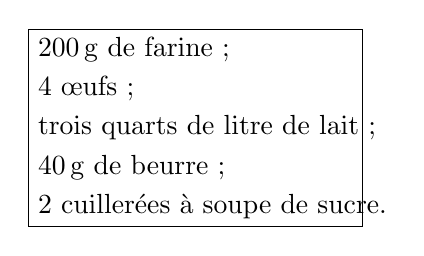
\begin{tikzpicture}[scale=0.5]
            \draw (0,0.5) rectangle (8.5,5.5);
            \node[anchor=west] at (0,5) {\qty{200}{\g} de farine ;};
            \node[anchor=west] at (0,4) {$4$ œufs ;};
            \node[anchor=west] at (0,3) {trois quarts de litre de lait ;};
            \node[anchor=west] at (0,2) {\qty{40}{\g} de beurre ;};
            \node[anchor=west] at (0,1) {$2$ cuillerées à soupe de sucre.};
        \end{tikzpicture}
        \end{center}
        \begin{sousitemize}
            \item Quelle quantité de farine est nécessaire pour $12$ personnes ?
            \item Pour $6$ personnes, combien faut-il de cuillerées de sucre ?
            \item Quelle quantité de beurre faut-il prévoir pour $7$ personnes ?
            \item Quelle quantité de lait faut-il prévoir pour $12$ personnes ?
        \end{sousitemize}
        \item L’élève sait exprimer un coefficient de proportionnalité sous la forme d’une fraction. Exemple :
        \begin{center}
        \begin{tabularx}{0.5\textwidth}{|X|c|}\hline
            Longueur du côté d'un carré avant agrandissement (\unit{\centi\metre}) & 3 \\\hline
            Longueur du côté d'un carré après agrandissement (\unit{\centi\metre}) & 7 \\\hline
        \end{tabularx}
        \end{center}
        \item Il sait donner un ordre de grandeur de $48 \%$ de \qty{60,45}{\EURO}.
        \item Il sait calculer $13 \%$ de \qty{225}{\EURO}.
        \item Il sait calculer mentalement
        \begin{sousitemize}
            \item $50 \%$ de $120$ élèves (la moitié, diviser par $2$)
            \item $25 \%$ de $120$ (le quart, diviser par $4$)
            \item $10 \%$ de $120$ (le dixième, diviser par $10$)
            \item $20 \%$ de $120$ ($2 \times 10 \%$, donc diviser par $10$ et multiplier par $2$)...
        \end{sousitemize}
        \item Un collège comporte $775$ élèves. $24 \%$ des élèves sont externes. Calcule le nombre d’élèves externes.

    \end{exemplesreussite}
    
    \clearpage
    \theme{GRANDEURS ET MESURES}
    \competence{Comparer, estimer, mesurer des grandeurs géométriques avec des nombres entiers et des nombres décimaux : longueur (périmètre), aire, volume, angle - Utiliser le lexique, les unités, les instruments de mesures spécifiques de ces grandeurs}
    \souscompetence{Longeurs}
    \begin{savoireleves}
        \item Il connaît la formule de la longueur d’un cercle et l’utilise.
    \end{savoireleves}
    \begin{exemplesreussite}
        \item Il calcule, à l’aide de la formule et en utilisant $3,14$ comme valeur approchée du nombre $\pi$, la longueur d’un cercle dont : 
        
        \begin{sousitemize}
            \item Le rayon est donné (par exemple par calcul mental dans le cas où le rayon est \qty{5}{\centi\metre}, ou à l’aide d’une multiplication posée ou de la calculatrice dans le cas où le rayon est de \qty{7,8}{\deci\metre})\\
            ($L_1 \approx 2 \times 3,14 \times \qty{5}{\centi\metre}$ et $L_2 \approx 2 \times 3,14 \times \qty{7,8}{\centi\metre}$)
            \item Le diamètre est donné (par exemple par calcul mental dans le cas où le diamètre est \qty{20}{\centi\metre}, ou à l’aide d’une multiplication posée ou de la calculatrice dans le cas où le diamètre est de \qty{9,6}{\centi\metre}).\\
            ($L_3 \approx 3,14 \times \qty{20}{\centi\metre}$ et $L_4 \approx 3,14 \times \qty{9,6}{m}$)
        \end{sousitemize}
        
        \begin{center}
        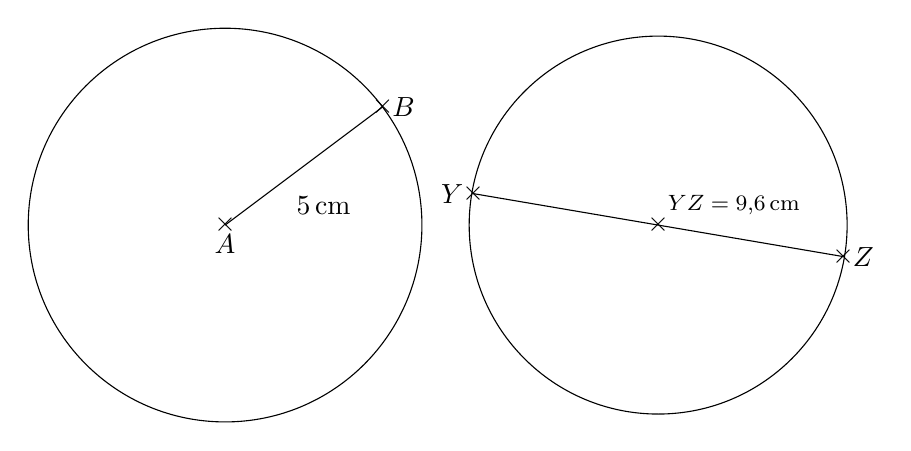
\begin{tikzpicture}[scale=0.5]
            \draw (0,0) circle (5);
            \draw (11,0) circle (4.8);
            \draw (0,0) node {$\times$} node[below] {$A$} -- (4,3) node {$\times$} node[right] {$B$};
            \node at (2.5,0.5) {\qty{5}{\centi\metre}};
            \draw (15.7,-0.8) node {$\times$} node[right] {$Z$} -- (11,0) node {$\times$} node[above right] {\footnotesize{$YZ=\qty{9,6}{\centi\metre}$}} -- (6.3,0.8) node {$\times$} node[left] {$Y$};
        \end{tikzpicture}
        \end{center}
        \centerline{\textit{Figures données à titre indicatif}}
        
        \item Il sait calculer des périmètres de figures composées de portions de cercle. Par exemple, il peut déterminer celui de la figure suivante :
        
        \begin{center}
        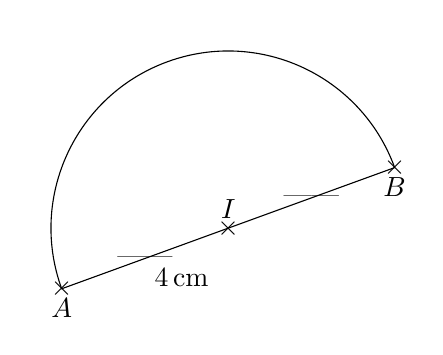
\begin{tikzpicture}[scale=1.5]
            \draw[rotate=20] (0,0) node {$\times$} node[below] {$B$} arc (0:180:1.5) node {$\times$} node[below] {$A$} -- (-2.25,0) node {||} node[below right] {\qty{4}{\centi\metre}} -- (-1.5,0) node {$\times$} node[above] {$I$} -- (-0.75,0) node {||} -- (0,0);
        \end{tikzpicture}
        \end{center}
        \centerline{\textit{Figure donnée à titre indicatif $\left(P \approx \qty{4}{\centi\metre} + \qty{4}{\centi\metre} + \left(3,14 \times \qty{8}{\centi\metre}\right) \div 2\right)$}}
    \end{exemplesreussite}
    
    \clearpage
    \souscompetence{Durées}
    \begin{savoireleves}
        \item Il réalise des conversions nécessitant deux étapes de traitement. (Transformer des heures en semaines, jours et heures ; transformer des secondes en heures, minutes, secondes).
    \end{savoireleves}
    
    \begin{exemplesreussite}
        \item Il transforme des heures en semaines, jours et heures :\\
        Combien font \qty{609}{\hour} en semaines, jours et heures ?
        \textit{($609$ heures correspondent à $3$ semaines $4$ jours et $9$ heures)}
        \item Il transforme des secondes en heures, minutes et secondes : \\
        Combien font \qty{34990}{\s} en heures, minutes et secondes ? 
        \textit{($9$ heures $43$ minutes et $10$ secondes).}
    \end{exemplesreussite}
    
    \souscompetence{Aires}
    \begin{savoireleves}
        \item Il utilise les multiples et sous-multiples du \unit{\metre\carre} et les relations qui les lient.
        \item Il calcule l’aire d’un triangle à l’aide de la formule.
        \item Il calcule l’aire d’un disque à l’aide de la formule.
        \item Il détermine la mesure de l’aire d’une surface.
    \end{savoireleves}
    
    \begin{exemplesreussite}
        \item Il sait que :
        \begin{sousitemize}
            \item \qty{1,5}{\kilo\metre\carre} correspond à \qty{1500000}{\metre\carre}
            \item \qty{10}{\metre\carre} correspondent à \qty{0,1}{\deca\metre\carre}
            \item \qty{45}{\centi\metre\carre} correspondent à \qty{0,0045}{\metre\carre}
            \item \qty{25}{\milli\metre\carre} correspondent à \qty{0,25}{\centi\metre\carre}
            \item \qty{3,12}{\deci\metre\carre} correspondent à \qty{312}{\centi\metre\carre}
        \end{sousitemize}
        
        \item \vspace{-2cm}
        \begin{minipage}[t]{0.5\textwidth}
            Il calcule l’aire d’un triangle rectangle, soit à l’aide de la formule de l’aire d’un triangle, soit en le considérant comme un « demi- rectangle ».\\
            \textit{(Par exemple, il peut calculer l’aire de la zone de jeux réservée pour les enfants en effectuant le calcul $\frac{\qty{30}{\metre} \times \qty{18}{\metre}}{2}$ qui donne \qty{270}{\metre\carre}.)}
        \end{minipage}\hspace{0.04\textwidth}
        \begin{minipage}{0.4\textwidth}
        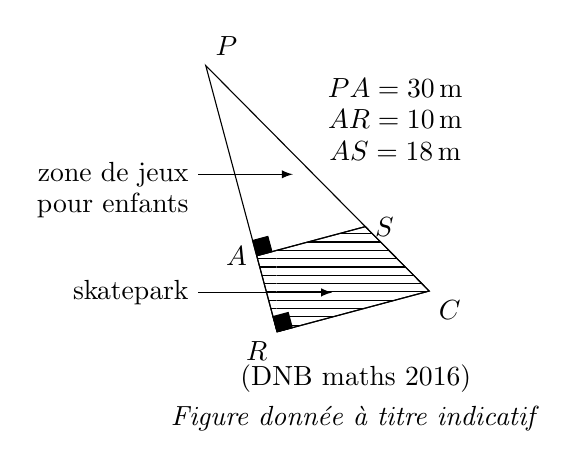
\begin{tikzpicture}
            \draw[rotate=15] (0,0) node[below left] {$R$} -- (2,0) node[below right] {$C$} -- (0,3.5) node[above right] {$P$} --cycle;
            \draw[rotate=15] (0,1) node[left] {$A$} -- ({10/7},1) node[right] {$S$};
            \draw[pattern=horizontal lines,rotate=15] (0,0) --  (0,1) -- ({10/7},1) -- (2,0) -- cycle;
            \node at (1.5,3.1) {$PA = \qty{30}{\metre}$};
            \node at (1.5,2.7) {$AR = \qty{10}{\metre}$};
            \node at (1.5,2.3) {$AS = \qty{18}{\metre}$};
            \node at (1,-0.6) {(DNB maths 2016)};
            \node at (1,-1.1) {\textit{Figure donnée à titre indicatif}};
            \draw[fill=black,rotate=15] (0,0) rectangle (0.2,0.2);
            \draw[fill=black,rotate=15] (0,1) rectangle (0.2,1.2);
            \draw[-latex] (-1,2) node[anchor=east] {zone de jeux} -- (0.2,2);
            \node[anchor=east] at (-1,1.6) {pour enfants};
            \draw[-latex] (-1,0.5) node[anchor=east] {skatepark} -- (0.7,0.5);
        \end{tikzpicture}
        \end{minipage}

        \vfill
        
        \item Il calcule, à l’aide de la formule, l’aire d’un triangle dans le cas où la hauteur est à l’intérieur du triangle en utilisant les données correctes. \\
        \textit{(Par exemple, il peut calculer l’aire du triangle $ABC$ suivant en effectuant le calcul $\frac{\qty{6}{\centi\metre} \times \qty{5,4}{\centi\metre}}{2}$ qui donne \qty{16,2}{\centi\metre\carre}.)}
        
        \begin{center}
        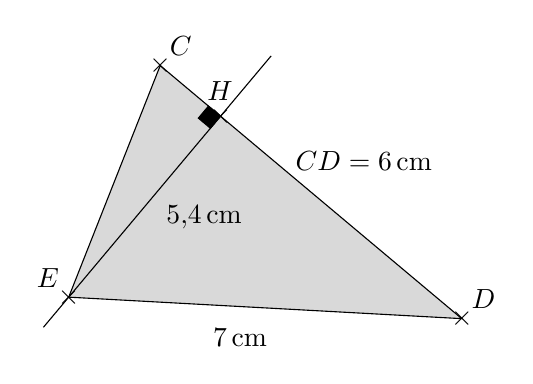
\begin{tikzpicture}
            \draw[fill=gray!30!white,rotate=140] (0,0) node {$\times$} (0.05,-0.05) node[above] {$H$} (0,0) -- (1,0) node {$\times$} node[above right] {$C$} -- (0,3) node {$\times$} node[above left] {$E$} -- (-4,0) node {$\times$} node[above right] {$D$} --cycle;
            \draw[rotate=140] (0,-1) -- (0,3.5) (-0.2,1.5) node[right] {\qty{5,4}{\centi\metre}};
            \draw[rotate=140] (-2,2) node {\qty{7}{\centi\metre}};
            \draw[rotate=140] (-1,-0.1) node[anchor=west] {$CD = \qty{6}{\centi\metre}$};
            \draw[fill=black,rotate=140] (0,0) rectangle (0.2,0.2);
        \end{tikzpicture}
        \end{center}
        \centerline{\textit{Figure donnée à titre indicatif}}
        
        \clearpage
        \item Il calcule, à l’aide de la formule, l’aire d’un triangle dans le cas où la hauteur donnée est à l’extérieur du triangle en utilisant les données correctes.\\
        \textit{(Par exemple, il peut calculer l’aire du triangle ABC suivant en effectuant le calcul $\frac{\qty{6}{\centi\metre} \times \qty{4}{\centi\metre}}{2}$ qui donne \qty{12}{\centi\metre\carre}.)}
        
        \begin{center}
        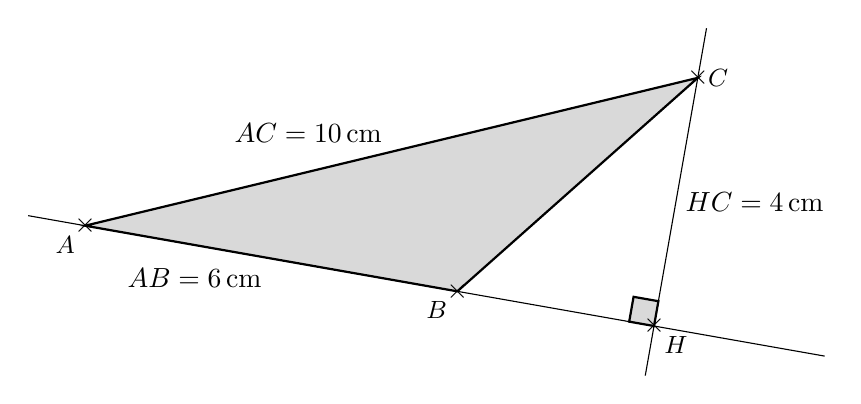
\begin{tikzpicture}[scale=0.8,rotate=-10]
            \coordinate (H) at (0,0);
            \coordinate (C) at (0,4);
            \coordinate (B) at (-3.17,0);
            \coordinate (A) at (-9.17,0);
            \draw ($(H)!-0.2!(C)$) -- ($(H)!1.2!(C)$);
            \draw ($(A)!-0.1!(H)$) -- ($(A)!1.3!(H)$);
            \draw[fill=gray!30!white,thick] (A) node{$\times$} node[below left]{\small{$A$}} -- (B) node{$\times$} node[below left]{\small{$B$}} -- (C) node{$\times$} node[right]{\small{$C$}} -- cycle;
            \draw[fill=gray!30!white,thick] (H) node{$\times$} node[below right]{\small{$H$}} rectangle ($(H)+(-0.4,0.4)$);
            \node[anchor=west] at ($(H)!0.5!(C)$) {$HC = \qty{4}{\centi\metre}$};
            \node[below left] at ($(A)!0.5!(B)$) {$AB = \qty{6}{\centi\metre}$};
            \node[above left] at ($(A)!0.5!(C)$) {$AC = \qty{10}{\centi\metre}$};
        \end{tikzpicture}
        \end{center}
        \centerline{\textit{Figure donnée à titre indicatif}}
        
        \item Il calcule, à l’aide de la formule et en utilisant une valeur approchée de $3,14$ pour le nombre $\pi$, l’aire d’un disque dont : 
        \begin{sousitemize}
            \item le rayon est donné \textit{(par exemple à l’aide d’une multiplication posée dans le cas où le rayon est de \qty{6}{\deci\metre} : $A_{\text{disque}} \approx 3,14 \times \qty{6}{\deci\metre} \times \qty{6}{\deci\metre}$ soit \qty{113,04}{\deci\metre\carre})}
            \item le diamètre est donné \textit{(par exemple à l’aide d’une multiplication posée dans le cas où le diamètre est de \qty{6}{\deci\metre} : $A_{\text{disque}} \approx 3,14 \times \qty{3}{\deci\metre} \times \qty{3}{\deci\metre}$ soit \qty{28,26}{\deci\metre\carre})}
        \end{sousitemize}
        
        \newcommand{\point}[2]{node{$\times$} node[#1]{#2}}

        \begin{center}
        \begin{tikzpicture}[scale=0.4]
            \draw (0,0) circle (3);
            \draw (10,0) circle (6);
            \draw (-2.598,-1.5) \point{below left}{$L$} -- (0,0) \point{above}{} -- (2.598,1.5) \point{above right}{$M$};
            \draw (10,0) \point{above left}{D} -- (15.196,3) \point{above right}{E};
            \node[rotate=30] at (12,2) {$DE=\qty{6}{\deci\metre}$};
            \node[rotate=30] at (-0.6,1) {$LM=\qty{6}{\deci\metre}$};
        \end{tikzpicture}
        \end{center}
        
        \centerline{\textit{Figures données à titre indicatif}}
        
        \item Il calcule l’aire d’une surface composée de figures simples (carré, rectangle, triangle). Par exemple, il détermine l’aire de la surface ci-dessous en effectuant la somme de l’aire d’un rectangle et de celle d’un triangle rectangle soit $(\qty{5}{\centi\metre} \times \qty{9}{\centi\metre}) + (\qty{8.4}{\centi\metre} - \qty{5}{\centi\metre}) \times (\qty{9}{\centi\metre} - \qty{4}{\centi\metre}) \div 2$ ce qui donne \qty{53.5}{\centi\metre\carre}.
        
        \begin{center}
        \begin{tikzpicture}[rotate=12,scale=0.6]
            \draw (0,0) -- (8.4,0) -- (5,5) -- (5,9) -- (0,9) -- cycle;
            \draw (0,0) rectangle (0.2,0.2) (0,9) rectangle (0.2,8.8) (5,9) rectangle (4.8,8.8);
            \node[anchor=north] at (4,-0.5) {\qty{8.4}{\centi\metre}};
            \node[anchor=east] at (0,4.5) {\qty{9}{\centi\metre}};
            \node[anchor=south] at (2,9) {\qty{5}{\centi\metre}};
            \node[anchor=west] at (5,7) {\qty{4}{\centi\metre}};
        \end{tikzpicture}
        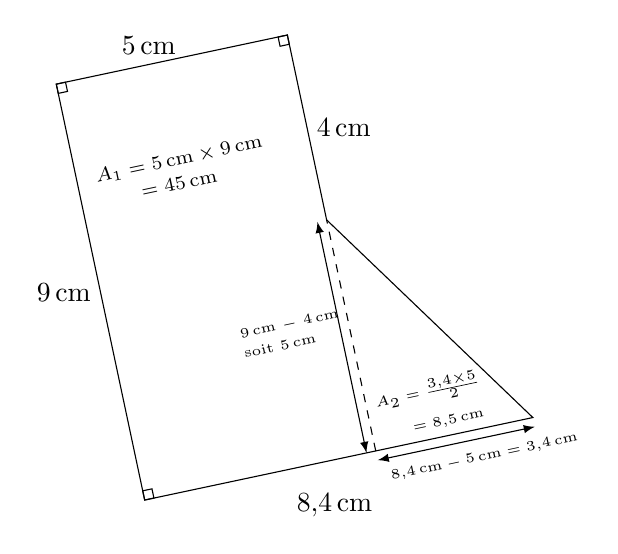
\begin{tikzpicture}[rotate=12,scale=0.6]
            \draw (0,0) -- (8.4,0) -- (5,5) -- (5,9) -- (0,9) -- cycle;
            \draw (0,0) rectangle (0.2,0.2) (0,9) rectangle (0.2,8.8) (5,9) rectangle (4.8,8.8);
            \node[anchor=north] at (4,-0.5) {\qty{8.4}{\centi\metre}};
            \node[anchor=east] at (0,4.5) {\qty{9}{\centi\metre}};
            \node[anchor=south] at (2,9) {\qty{5}{\centi\metre}};
            \node[anchor=west] at (5,7) {\qty{4}{\centi\metre}};
            \node[rotate=12,anchor=west] at (0.2,6.9) {\scriptsize{$\mathscr{A}_1 = \qty{5}{\centi\metre} \times \qty{9}{\centi\metre}$}};
            \node[rotate=12,anchor=west] at (0.45,6.4) {\scriptsize{$~~~~=\qty{45}{\centi\metre\carre}$}};
            \draw[dashed] (5,0) -- (5,5);
            \draw[latex-latex] (4.8,0) -- (4.8,5);
            \node[rotate=12,anchor=west] at (2.5,3) {\tiny{\qty{9}{\centi\metre} $-$ \qty{4}{\centi\metre}}};
            \node[rotate=12,anchor=west] at (2.5,2.6) {\tiny{soit $\qty{5}{\centi\metre}$}};
            \draw[latex-latex] (5,-0.2) -- (8.4,-0.2);
            \node[rotate=12,anchor=west] at (5,-0.6) {\tiny{$\qty{8.4}{\centi\metre} - \qty{5}{\centi\metre} = \qty{3.4}{\centi\metre}$}};
            \node[rotate=12,anchor=west] at (5,1) {\tiny{$\mathscr{A}_2 = \frac{3,4 \times 5}{2}$}};
            \node[rotate=12,anchor=west] at (5.67,0.3) {\tiny{$=\qty{8,5}{\centi\metre\carre}$}};
        \end{tikzpicture}
        \end{center}
        \centerline{\textit{Figures données à titre indicatif}}
        \clearpage

        \item Il calcule l’aire d’une surface composée de figures simples (dont des disques). Par exemple, il peut déterminer l’aire de la surface grisée de la figure suivante, en sachant que le rayon d’un disque blanc est de \qty{4}{\centi\metre}.
        
        \begin{center}
        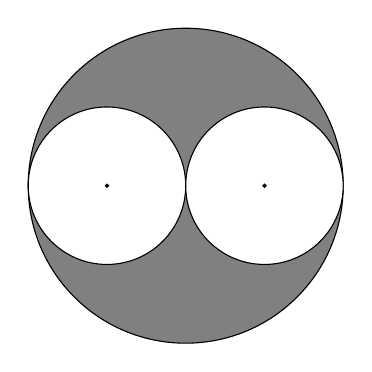
\begin{tikzpicture}
            \draw[fill=gray] (0,0) circle (2);
            \draw[fill=white] (-1,0) circle (1);
            \draw[fill=white] (1,0) circle (1);
            \draw[fill=black] (-1,0) circle (0.02) (1,0) circle (0.02);
        \end{tikzpicture}
        \end{center}

        $\mathscr{A}_{\text{surface grisée}} \approx \left(3,14 \times \qty{8}{\centi\metre} \times \qty{8}{\centi\metre} \right) - 2 \times \left( 3,14 \times \qty{4}{\centi\metre} \times \qty{4}{\centi\metre} \right)$ soit \qty{100,48}{\centi\metre\carre}.
    \end{exemplesreussite}
    
    \souscompetence{Contenances et volumes}
    \begin{savoireleves}
        \item Il calcule le volume d’un cube ou d’un pavé droit en utilisant une formule.
        \item Il utilise les unités de volume : \unit{\centi\metre\cube}, \unit{\deci\metre\cube} et \unit{\metre\cube} et leurs relations.
        \item Il relie les unités de volume et de contenance ($\qty{1}{\litre} = \qty{1}{\deci\metre\cube}$ ; $\qty{1000}{\litre} = \qty{1}{\metre\cube}$).
    \end{savoireleves}
    
    \begin{exemplesreussite}
        \item[\CR] Un pavé droit a pour longueur \qty{30}{\centi\metre}, pour largeur \qty{25}{\centi\metre} et pour hauteur \qty{15}{\centi\metre}. Calcule son volume en \unit{\centi\metre\cube} puis en \unit{\deci\metre\cube}. \textit{(Réponse : il peut effectuer le calcul $\qty{30}{\centi\metre} \times \qty{25}{\centi\metre} \times \qty{15}{\centi\metre}$ qui donne \qty{11250}{\centi\metre\cube}, soit \qty{11,25}{\deci\metre\cube}.)}
        \item[\CR] Pierre plonge un premier cube fermé de \qty{15}{\centi\metre} de côté dans une bassine remplie d’eau à ras bord.
        \begin{sousitemize}
            \item Indique, en \unit{\litre}, la quantité d’eau qui sera récupérée hors de la bassine.
            \item Il remplit à nouveau la bassine à ras bord et plonge cette fois-ci un cube de \qty{2,5}{\centi\metre} de côté. Indique, en \unit{\milli\litre}, la quantité d’eau récupérée hors de la bassine.
        \end{sousitemize}
    \end{exemplesreussite}
    
    \souscompetence{Angles}
    \begin{savoireleves}
        \item Il estime si un angle est droit, aigu ou obtus.
        \item Il utilise un rapporteur pour mesurer un angle en degrés.
        \item Il construit, à l’aide du rapporteur, un angle de mesure donnée en degrés.
    \end{savoireleves}
    
    \begin{exemplesreussite}
        \item Il mesure un angle dont le rapporteur est déjà correctement positionné.
        
        \begin{center}
        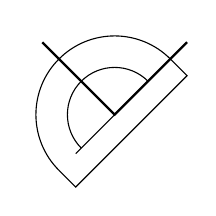
\begin{tikzpicture}[rotate=45]
            \draw (-0.7,0) -- (0.7,0);
            \draw (-1,0) -- (-1,-0.3) -- (1,-0.3) -- (1,0);
            \draw (1,0) arc (0:180:1);
            \draw (0.6,0) arc (0:180:0.6);
            \directlua{
                for d = 0,180,10
                do 
                    n = math.rad(d)
                    r1, r2, r3, r4 = 0.6, 0.67, 0.9, 1
                    x1, y1, x2, y2 = r1*math.cos(n), r1*math.sin(n), r2*math.cos(n), r2*math.sin(n)
                    x3, y3, x4, y4 = r3*math.cos(n), r3*math.sin(n), r4*math.cos(n), r4*math.sin(n)
                    tex.sprint("\\draw (", x1, ",", y1, ") -- (", x2, ",", y2, ");")
                    tex.sprint("\\draw (", x3, ",", y3, ") -- (", x4, ",", y4, ");")
                end
            }
            \draw[thick] (0,1.3) -- (0,0) -- (1.3,0);
        \end{tikzpicture}
        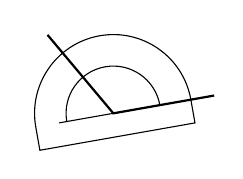
\begin{tikzpicture}[rotate=10]
            \draw (-0.7,0) -- (0.7,0);
            \draw (-1,0) -- (-1,-0.3) -- (1,-0.3) -- (1,0);
            \draw (1,0) arc (0:180:1);
            \draw (0.6,0) arc (0:180:0.6);
            \directlua{
                for d = 0,180,10
                do 
                    n = math.rad(d)
                    r1, r2, r3, r4 = 0.6, 0.67, 0.9, 1
                    x1, y1, x2, y2 = r1*math.cos(n), r1*math.sin(n), r2*math.cos(n), r2*math.sin(n)
                    x3, y3, x4, y4 = r3*math.cos(n), r3*math.sin(n), r4*math.cos(n), r4*math.sin(n)
                    tex.sprint("\\draw (", x1, ",", y1, ") -- (", x2, ",", y2, ");")
                    tex.sprint("\\draw (", x3, ",", y3, ") -- (", x4, ",", y4, ");")
                end
            }
            \draw[thick] (-0.65,1.126) -- (0,0) -- (1.3,0);
        \end{tikzpicture}
        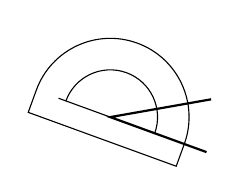
\begin{tikzpicture}[rotate=-20]
            \draw (-0.7,0) -- (0.7,0);
            \draw (-1,0) -- (-1,-0.3) -- (1,-0.3) -- (1,0);
            \draw (1,0) arc (0:180:1);
            \draw (0.6,0) arc (0:180:0.6);
            \directlua{
                for d = 0,180,10
                do 
                    n = math.rad(d)
                    r1, r2, r3, r4 = 0.6, 0.67, 0.9, 1
                    x1, y1, x2, y2 = r1*math.cos(n), r1*math.sin(n), r2*math.cos(n), r2*math.sin(n)
                    x3, y3, x4, y4 = r3*math.cos(n), r3*math.sin(n), r4*math.cos(n), r4*math.sin(n)
                    tex.sprint("\\draw (", x1, ",", y1, ") -- (", x2, ",", y2, ");")
                    tex.sprint("\\draw (", x3, ",", y3, ") -- (", x4, ",", y4, ");")
                end
            }
            \draw[thick] (1.126,0.65) -- (0,0) -- (1.3,0);
        \end{tikzpicture}
        \end{center}
        
        \item Il mesure un angle avec son propre rapporteur.
        
        \begin{center}
        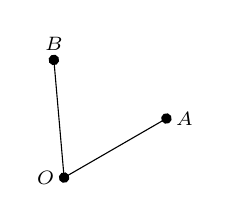
\begin{tikzpicture}[rotate=30,scale=1.5]
            \coordinate (O) at (0,0);
            \coordinate (A) at (1,0);
            \coordinate (B) at (0.423,0.906);
            \draw (A) -- (O) -- (B);
            \draw[fill=black] (A) circle (0.04) node[right] {\scriptsize{$A$}};
            \draw[fill=black] (O) circle (0.04) node[left] {\scriptsize{$O$}};
            \draw[fill=black] (B) circle (0.04) node[above] {\scriptsize{$B$}};
        \end{tikzpicture}
        \begin{tikzpicture}[rotate=-20,scale=1.5]
            \coordinate (I) at (0,0);
            \coordinate (C) at (1,0);
            \coordinate (D) at (-0.866,0.5);
            \draw (C) -- (I) -- (D);
            \draw[fill=black] (C) circle (0.04) node[right] {\scriptsize{$C$}};
            \draw[fill=black] (I) circle (0.04) node[below left] {\scriptsize{$I$}};
            \draw[fill=black] (D) circle (0.04) node[above] {\scriptsize{$D$}};
        \end{tikzpicture}
        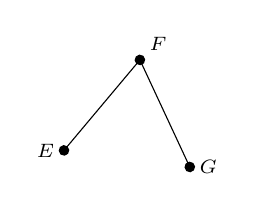
\begin{tikzpicture}[rotate=-130,scale=1.5]
            \coordinate (F) at (0,0);
            \coordinate (E) at (1,0);
            \coordinate (G) at (0.423,0.906);
            \draw (E) -- (F) -- (G);
            \draw[fill=black] (E) circle (0.04) node[left] {\scriptsize{$E$}};
            \draw[fill=black] (F) circle (0.04) node[above right] {\scriptsize{$F$}};
            \draw[fill=black] (G) circle (0.04) node[right] {\scriptsize{$G$}};
        \end{tikzpicture}
        \end{center}
        
        \centerline{$\widehat{AOB} = 65$° ~~~~ $\widehat{CID} = 150$° ~~~~ $\widehat{EFG} = 90$°}
        
        \item[\CR] Construis un angle $\widehat{AOB}$ de mesure 70° et un angle $\widehat{COD}$ de mesure 150°.
    \end{exemplesreussite}
    
    \clearpage
    \competence{Résoudre des problèmes impliquant des grandeurs (géométriques, physiques, \\économiques) en utilisant des nombres entiers et des nombres décimaux}
    
    \begin{savoireleves}
        \item Dès le CM1, les élèves commencent à identifier et à résoudre des problèmes de proportionnalité portant sur des grandeurs.
        \item À partir du CM2, des situations simples impliquant des échelles et des vitesses constantes peuvent être rencontrées.
    \end{savoireleves}
    
    \begin{exemplesreussite}
        \item[] \textbf{\textit{Problèmes additifs}}
        \item Il peut additionner ou soustraire des nombres associés à des grandeurs
        \item[\CR] Un vase pouvant contenir \qty{2}{\litre} contient déjà \qty{1,3}{\litre} d’eau. Si on verse à nouveau \qty{50}{\centi\litre}, l’eau débordera-t-elle ?\\
        \textit{(Réponse : Non car $\qty{50}{\centi\litre} = \qty{0,5}{\centi\litre}$ et que $\qty{1,3}{\litre} + \qty{0,5}{\litre} = \qty{1,8}{\litre}.$)}
        \item[\CR] Sohan et sa famille sont partis à 8h50 de leur domicile. Ils sont arrivés à 20h15 sur leur lieu de vacances. Combien de temps a duré leur voyage ?\\
        \textit{(Réponse : 11h25min)}
        \item[] \textbf{\textit{Problèmes multiplicatifs}}
        \item[] \textit{Problèmes de proportion simple}
        \item[\CR] Un robinet mal fermé laisse échapper \qty{1}{\milli\litre} d’eau toutes les \qty{10}{\s}. Est-ce vrai que cela représente plus de \qty{8}{\litre} d’eau perdue par jour ? (Réponse : Oui, car le robinet laisse échapper \qty{6}{\milli\litre} en 1 min soit \qty{360}{\milli\litre} en 1h d’où \qty{8640}{\milli\litre} (\qty{8.64}{\litre}) en 24h.)
        \item[\CR] Quelle est la longueur du côté d’un terrain carré de périmètre \qty{18}{\metre} ? Et de périmètre \qty{23.2}{\metre} ?\\
        \textit{(Réponse : $\qty{18}{\metre} \div 4 = \qty{4.5}{\metre}$ et $\qty{23.2}{\metre} \div 4 = \qty{5.8}{\metre}$.)}
        \item[\CR] Quelle est la longueur du rayon d’un cercle de périmètre $\qty{62.8}{\deci\metre}$ ?\\
        \textit{(Réponse : la longueur d’un cercle de rayon $r$ étant donné par la formule $2 \times \pi \times r$, il faut faire le calcul $62,8 \div \left(2 \times \pi\right)$ qui donne environ \qty{10}{\deci\metre}.)}
        \item[\CR] Un pack contient $6$ bouteilles de \qty{1.5}{\litre} de jus d’orange. Combien de gobelets de \qty{20}{\centi\litre}, pleins à ras bord, peut-on espérer servir ?\\
        \textit{(Réponse : $45$ gobelets car $\qty{1.5}{\litre} = \qty{150}{\centi\litre}$ et que la division euclidienne de $900$ par $20$ donne $45$ comme quotient et zéro comme reste.)}
        \item[\CR] Pour remplir $4$ aquariums identiques, \qty{128}{\deci\metre\cube} d’eau ont été nécessaires. Quelle quantité d’eau faudrait-il pour remplir $10$ aquariums de même volume que les précédents ?\\
        \textit{(Réponse : \qty{320}{\deci\metre\cube}, puisqu’il faut \qty{32}{\deci\metre\cube} par aquarium.)} 
        \item[] \textit{Problèmes de comparaison du type « fois plus, fois moins »}
        \item[\CR] Myriam a dépensé \qty{85.56}{\EURO} en frais d’essence ce mois-ci. Flora a dépensé trois fois moins qu’elle ; à combien lui reviennent ses dépenses ? (Réponse : $\qty{85.56}{\EURO} \div 3 = \qty{28.52}{\EURO}$.) 
        \item[] \textit{Problèmes de produit de mesures}
        \item[\CR] Selon l’INSEE, la Guadeloupe possède une superficie de \qty{1703}{\kilo\metre\carre} et une densité, en $2011$, de population de $238$ habitants par \unit{\kilo\metre\carre}. Quel est le nombre d’habitants en Guadeloupe en $2011$ ? \\
        \textit{(Réponse : $\qty{1703}{\kilo\metre\carre} \times \qty{238}{habitants\per\kilo\metre\carre} = \qty{405314}{habitants}$.)}
        \item[\CR] Quelle est la longueur du côté d’un terrain carré d’aire \qty{25}{\metre\carre} ? (Réponse : \qty{5}{\metre}.)
        \item[\CR] Yasmine roule à une vitesse constante de \qty{20}{\kilo\metre\per\hour} sur son vélo. Quelle distance, au dixième de kilomètre près, a-t-elle parcourue à la fin de son parcours d’une heure et quarante minutes ?\\
        \textit{(Réponse : \qty{33.3}{\kilo\metre}.)}
    \end{exemplesreussite}
    
    \clearpage
    \theme{ESPACE ET GÉOMÉTRIE}
    \competence{(Se) repérer et (se) déplacer dans l’espace en utilisant ou en élaborant des représentations}
    
    \begin{savoireleves}
        \item[] \textbf{\textit{Dans divers modes de représentation de l’espace (maquettes, plans, schémas)}}
        \item Il se repère, décrit (tourner à gauche, à droite ; faire demi-tour ; effectuer un quart de tour à droite, à gauche) ou exécute des déplacements.
        \item Il connaît et programme des déplacements absolus (vers le haut, l’ouest...) d’un robot ou ceux d’un personnage sur un écran.
        \item Il connaît et programme des déplacements relatifs (tourner à sa gauche, à sa droite ; faire demi-tour ; effectuer un quart de tour à sa droite, à sa gauche...) d’un robot ou ceux d’un personnage sur un écran.
    \end{savoireleves}
    
    \begin{exemplesreussite}
        \item Sur le plan suivant qui représente un espace familier (village mais cela aurait pu être son école, son quartier, sa ville), il est capable de dire que la mairie se trouve en $(4;3)$.\\
        Il est capable de représenter un trajet de la mairie au théâtre.\\
        Il est capable de décrire le déplacement à effectuer. (Aller vers la place de Lattre Tassigny, puis prendre la 3\textsuperscript{e} rue à votre gauche...)
        
        \begin{figure}[h!]
            \centering
            \begin{tikzpicture}[scale=0.8]
                \node[anchor=south west] at (0,0) {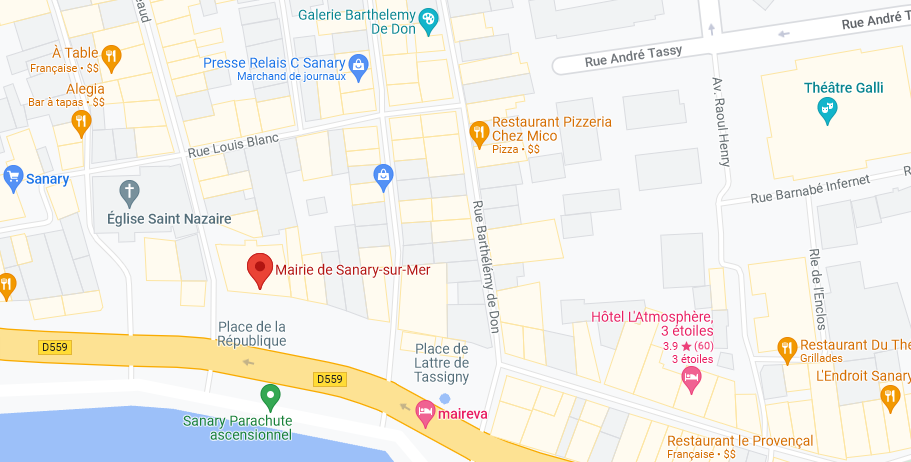
\includegraphics[scale=0.44]{Programmes du B.O./Collège/sanary_sur_mer.PNG}};
                \draw[-latex] (0,0) -- (14,0);
                \draw[-latex] (0,0) -- (0,7);
                \foreach \x in {0,1,...,13} {
                    \draw (\x,0) -- (\x,0.2);
                    \node[below] at (\x,0) {$\x$};
                }
                \foreach \y in {1,2,...,7} {
                    \draw (0,{0.9*\y}) -- (0.2,{0.9*\y});
                    \node[left] at (0,{0.9*\y}) {$\y$};
                }
            \end{tikzpicture}
        \end{figure}
        
        \item À l’aide d’un logiciel de programmation, la situation suivante étant donnée, il est capable d’assembler des blocs de déplacements pour faire sortir la balle du labyrinthe et de décrire le trajet effectué.
        \item À l’aide d’un logiciel de programmation, la situation ci-contre étant donnée, il est capable de créer des commandes pour déplacer la balle à l’intérieur du labyrinthe.
        \item Il complète le programme ci-dessous à l’aide des blocs afin d’obtenir la frise :
        
        \begin{center}
        \begin{tikzpicture}
            \node[anchor=west] at (0,0) {%
                \begin{tikzpicture}[scale=0.7]
                    \draw (0,1) -- (0,0) -- (1,0) -- (1,1) -- (2,1) -- (2,0) -- (3,0) -- (3,1) -- (4,1) -- (4,0) -- (5,0) -- (5,1) -- (6,1) -- (6,0) -- (7,0) -- (7,1) -- (8,1);
                    \node[anchor=west] at (8,1) {
\includegraphics[scale=0.15]{Programmes du B.O./Collège/lutin.png}};
                \end{tikzpicture}%
            };
            \node[anchor=east] at (-1,0) {%
                \begin{scratch}[scale=0.6]
                    \blockinit{quand \greenflag est cliqué}
                    \blockpen{effacer tout}
                    \blockpen{mettre à \ovalnum{50} \% de la taille initiale}
                    \blockmove{s'orienter à \ovalnum{90}°}
                    \blockmove{aller à x:\ovalnum{-200} y:\ovalnum{0}}
                    \blockpen{stylo en position d'écriture}
                    \blockmove{tourner \turnright{} de \ovalnum{90} degrés}
                    \blockmove{avancer de \ovalnum{30}}
                    \blockmove{tourner \turnleft{} de \ovalnum{90} degrés}
                \end{scratch}%
            };
        \end{tikzpicture}
        \end{center}
    \end{exemplesreussite}
    
    \competence{Reconnaître, nommer, décrire, reproduire, représenter, construire des solides et figures géométriques}
    \souscompetence{Reconnaître, nommer, décrire}
    
    \begin{savoireleves}
        \item[] \textit{Dans le plan}
        \item Il code des figures simples :
        \begin{sousitemize}
            \item les triangles (dont les triangles particuliers : triangle rectangle, isocèle, équilatéral) ;
            \item les quadrilatères (dont les quadrilatères particuliers : carré, rectangle, losange).
        \end{sousitemize}
        \item Il connaît et utilise le vocabulaire associé à ces figures et à leurs propriétés (côté, sommet, angle, diagonale, polygone, centre, rayon, diamètre, milieu, hauteur) pour décrire et coder ces figures.
        \item Il reconnaît, nomme et décrit des figures complexes (assemblages de figures simples).
        \item[] \textit{Dans l'espace}
        \item Il reconnaît, nomme et décrit des assemblages de solides simples.
    \end{savoireleves}
    
    \begin{exemplesreussite}
        \item[] \textit{Dans le plan}
        \item Il est capable de coder les figures comme ci-dessous pour traduire qu’elles représentent un triangle rectangle, un triangle isocèle en $L$, un triangle équilatéral, un rectangle, un losange, un carré.

        \begin{center}
        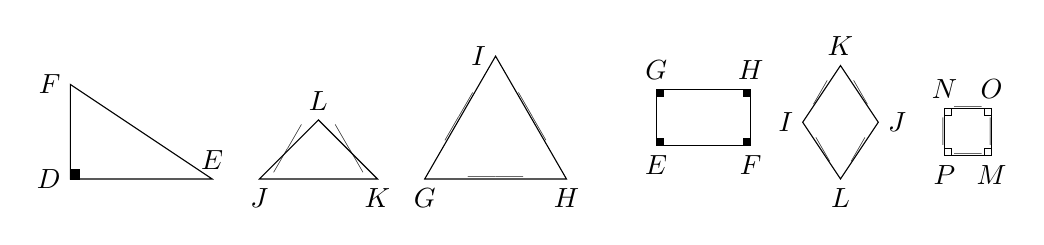
\begin{tikzpicture}[scale=0.6]
            \coordinate (D) at (-2,0);
            \coordinate (E) at (1,0);
            \coordinate (F) at (-2,2);
            \draw (D) -- (E) -- (F) -- cycle;
            \node[left] at (D) {$D$};
            \node[above] at (E) {$E$};
            \node[left] at (F) {$F$};
            \draw[fill=black] (D) rectangle ($(D)+(0.2,0.2)$);

            \coordinate (J) at (2,0);
            \coordinate (K) at (4.5,0);
            \coordinate (L) at (3.25,1.25);
            \draw (J) -- (K) -- (L) -- cycle;
            \node[below] at (J) {$J$};
            \node[below] at (K) {$K$};
            \node[above] at (L) {$L$};

            \node[rotate=60] at ($(J)!0.5!(L)$) {||};
            \node[rotate=-60] at ($(K)!0.5!(L)$) {||};

            \coordinate (G) at (5.5,0);
            \coordinate (H) at (8.5,0);
            \coordinate (I) at (7,2.6);
            \draw (G) -- (H) -- (I) -- cycle;
            \node[below] at (G) {$G$};
            \node[below] at (H) {$H$};
            \node[left] at (I) {$I$};

            \node[rotate=60] at ($(G)!0.5!(I)$) {||};
            \node at ($(G)!0.5!(H)$) {||};
            \node[rotate=-60] at ($(I)!0.5!(H)$) {||};
            
            \coordinate (E) at (10.4,0.7);
            \coordinate (F) at (12.4,0.7);
            \coordinate (H) at (12.4,1.9);
            \coordinate (G) at (10.4,1.9);
            \draw (E) -- (F) -- (H) -- (G) -- cycle;
            \draw[fill=black] (E) rectangle ($(E)+(0.15,0.15)$);
            \draw[fill=black] (F) rectangle ($(F)+(-0.15,0.15)$);
            \draw[fill=black] (H) rectangle ($(H)+(-0.15,-0.15)$);
            \draw[fill=black] (G) rectangle ($(G)+(0.15,-0.15)$);

            \node[below] at (E) {$E$};
            \node[below] at (F) {$F$};
            \node[above] at (H) {$H$};
            \node[above] at (G) {$G$};
            
            \coordinate (I) at (13.5,1.2);
            \coordinate (J) at (15.1,1.2);
            \coordinate (L) at (14.3,0);
            \coordinate (K) at (14.3,2.4);
            \draw (I) -- (L) -- (J) -- (K) -- cycle;
            \node[left] at (I) {$I$};
            \node[right] at (J) {$J$};
            \node[above] at (K) {$K$};
            \node[below] at (L) {$L$};

            \node[rotate=60] at ($(I)!0.5!(K)$) {|};
            \node[rotate=-60] at ($(K)!0.5!(J)$) {|};
            \node[rotate=60] at ($(J)!0.5!(L)$) {|};
            \node[rotate=-60] at ($(I)!0.5!(L)$) {|};
            
            \coordinate (N) at (16.5,1.5);
            \coordinate (O) at (17.5,1.5);
            \coordinate (M) at (17.5,0.5);
            \coordinate (P) at (16.5,0.5);
            \draw (N) -- (O) -- (M) -- (P) -- cycle;
            \draw (N) rectangle ($(N) + (0.15,-0.15)$);
            \draw (O) rectangle ($(O) + (-0.15,-0.15)$);
            \draw (M) rectangle ($(M) + (-0.15,0.15)$);
            \draw (P) rectangle ($(P) + (0.15,0.15)$);
            \node[above] at (N) {$N$};
            \node[above] at (O) {$O$};
            \node[below] at (M) {$M$};
            \node[below] at (P) {$P$};

            \node at ($(N)!0.5!(O)$) {|};
            \node[rotate=90] at ($(O)!0.5!(M)$) {|};
            \node at ($(P)!0.5!(M)$) {|};
            \node[rotate=90] at ($(P)!0.5!(N)$) {|};
        \end{tikzpicture}
        \end{center}
        
        \item Il reconnaît ces triangles à l’aide d’une figure codée ou renseignée : Il est capable de dire que dans la configuration suivante le triangle $ADB$ est un triangle isocèle en $A$ car $AD = AB$.
        
        \begin{center}
        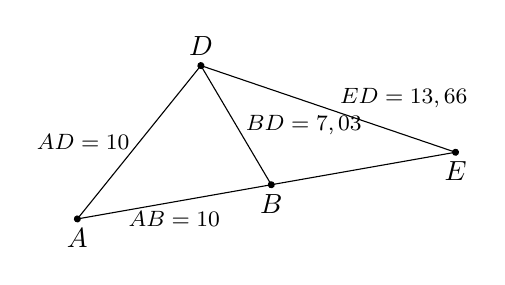
\begin{tikzpicture}[rotate=10,scale=0.25]
            \coordinate (A) at (0,0);
            \coordinate (B) at (10,0);
            \coordinate (E) at (19.5,0);
            \coordinate (D) at (7.53,6.58);
            \draw (B) -- (D) -- (A) -- (E) -- (D);
            \draw[fill=black] (B) circle (0.15);
            \draw[fill=black] (A) circle (0.15);
            \draw[fill=black] (E) circle (0.15);
            \draw[fill=black] (D) circle (0.15);
            \node[below] at (B) {$B$};
            \node[below] at (A) {$A$};
            \node[below] at (E) {$E$};
            \node[above] at (D) {$D$};
            \node[anchor=east] at ($(A)!0.5!(D)$) {\footnotesize{$AD=10$}};
            \node[anchor=north] at ($(A)!0.5!(B)$) {\footnotesize{$AB=10$}};
            \node[anchor=west] at ($(B)!0.5!(D)$) {\footnotesize{$BD=7,03$}};
            \node[anchor=west] at ($(D)!0.5!(E)+(0.2,0.5)$) {\footnotesize{$ED=13,66$}};
        \end{tikzpicture}
        \end{center}
        
        \item Il est capable de dire que le point $A$ appartient au disque de centre $O$ et de rayon $[OB]$, que le point $B$ appartient au cercle de centre $O$ et de rayon $[OB]$ et que le point $D$ n’appartient ni à l’un ni à l’autre.

        \begin{center}
        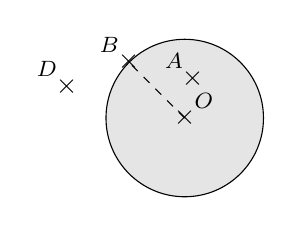
\begin{tikzpicture}
            \draw[fill=gray!20!white] (0,0) circle (1);
            \draw (0,0) node{$\times$} node[above right] {\footnotesize{$O$}};
            \draw (0.1,0.5) node{$\times$} node[above left] {\footnotesize{$A$}};
            \draw (-0.714,0.714) node{$\times$} node[above left] {\footnotesize{$B$}};
            \draw (-1.5,0.4) node{$\times$} node[above left] {\footnotesize{$D$}};
            \draw[dashed] (0,0) -- (-0.714,0.714);
        \end{tikzpicture}
        \end{center}

        
        \item Il est capable de dire que le triangle $IJK$ étant isocèle en $L$, ses angles à la base ont la même mesure ou que le triangle $IGH$ étant équilatéral, ses angles ont tous la même mesure.

        \begin{center}
        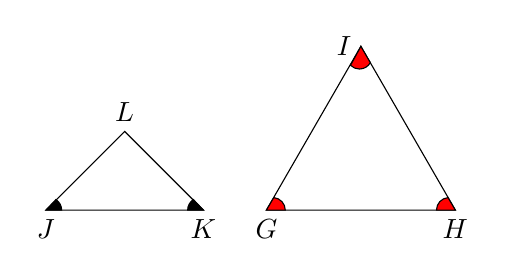
\begin{tikzpicture}[scale=0.8]
            \coordinate (J) at (2,0);
            \coordinate (K) at (4.5,0);
            \coordinate (L) at (3.25,1.25);
            \draw (J) -- (K) -- (L) -- cycle;
            \node[below] at (J) {$J$};
            \node[below] at (K) {$K$};
            \node[above] at (L) {$L$};

            \draw[fill=black] ($(J)!0.1!(K)$) arc (0:57:0.2) -- (J) -- cycle;
            \draw[fill=black] ($(K)!0.1!(J)$) arc (180:123:0.2) -- (K) -- cycle;

            \coordinate (G) at (5.5,0);
            \coordinate (H) at (8.5,0);
            \coordinate (I) at (7,2.6);
            \draw (G) -- (H) -- (I) -- cycle;
            \node[below] at (G) {$G$};
            \node[below] at (H) {$H$};
            \node[left] at (I) {$I$};

            \draw[fill=red] ($(G)!0.1!(H)$) arc (0:85:0.2) -- (G) -- cycle;
            \draw[fill=red] ($(H)!0.1!(G)$) arc (180:95:0.2) -- (H) -- cycle;
            \draw[fill=red] ($(I)!0.1!(H)$) arc (-30:-135:0.2) -- (I) -- cycle;
        \end{tikzpicture}
        \end{center}

        \clearpage
        \item Il est capable de dire que $GHFE$ étant un rectangle, ses diagonales $[GF]$ et $[HE]$ se coupent en leur milieu et ont la même mesure.

        \begin{center}
        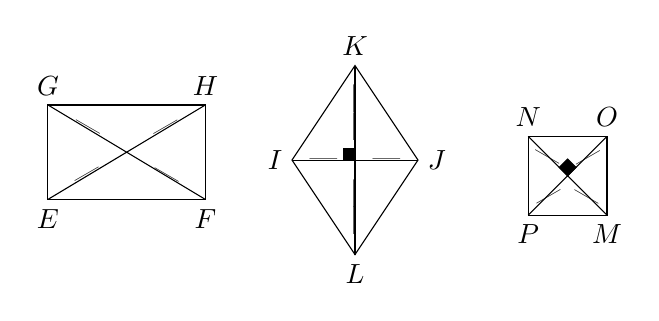
\begin{tikzpicture}
            \coordinate (E) at (10.4,0.7);
            \coordinate (F) at (12.4,0.7);
            \coordinate (H) at (12.4,1.9);
            \coordinate (G) at (10.4,1.9);
            \coordinate (O) at ($(G)!0.5!(F)$);
            \draw (E) -- (F) -- (H) -- (G) -- cycle;
            \draw (E) -- (H) (G) -- (F);

            \node[below] at (E) {$E$};
            \node[below] at (F) {$F$};
            \node[above] at (H) {$H$};
            \node[above] at (G) {$G$};
            \node[rotate=30] at ($(E)!0.5!(O)$) {|};
            \node[rotate=-30] at ($(F)!0.5!(O)$) {|};
            \node[rotate=30] at ($(H)!0.5!(O)$) {|};
            \node[rotate=-30] at ($(G)!0.5!(O)$) {|};
            
            \coordinate (I) at (13.5,1.2);
            \coordinate (J) at (15.1,1.2);
            \coordinate (L) at (14.3,0);
            \coordinate (K) at (14.3,2.4);
            \coordinate (O) at ($(I)!0.5!(J)$);
            \draw (I) -- (L) -- (J) -- (K) -- cycle;
            \draw (I) -- (J) (L) -- (K);
            \node[left] at (I) {$I$};
            \node[right] at (J) {$J$};
            \node[above] at (K) {$K$};
            \node[below] at (L) {$L$};

            \node[rotate=0] at ($(I)!0.5!(O)$) {|};
            \node[rotate=0] at ($(J)!0.5!(O)$) {|};
            \node[rotate=90] at ($(K)!0.5!(O)$) {||};
            \node[rotate=90] at ($(L)!0.5!(O)$) {||};
            \draw[fill=black] (O) rectangle ($(O)+(-0.15,0.15)$);
            
            \coordinate (N) at (16.5,1.5);
            \coordinate (O) at (17.5,1.5);
            \coordinate (M) at (17.5,0.5);
            \coordinate (P) at (16.5,0.5);
            \coordinate (C) at ($(N)!0.5!(M)$);
            \draw (N) -- (O) -- (M) -- (P) -- cycle;
            \draw (N) -- (M) (O) -- (P);

            \node[rotate=150] at ($(N)!0.5!(C)$) {|};
            \node[rotate=-150] at ($(O)!0.5!(C)$) {|};
            \node[rotate=150] at ($(M)!0.5!(C)$) {|};
            \node[rotate=-150] at ($(P)!0.5!(C)$) {|};
            \draw[fill=black,rotate=45] (C) rectangle ($(C)+(0.15,0.15)$);

            \node[above] at (N) {$N$};
            \node[above] at (O) {$O$};
            \node[below] at (M) {$M$};
            \node[below] at (P) {$P$};
        \end{tikzpicture}
        \end{center}

        \item Il est capable, à l’aide de n’importe laquelle des représentations suivantes, de dire que le segment $[AH]$ est la hauteur issue de $A$ du triangle $ABC$ et que la longueur de ce segment représente donc la distance du point $A$ à la droite $(BC)$.

        \begin{center}
        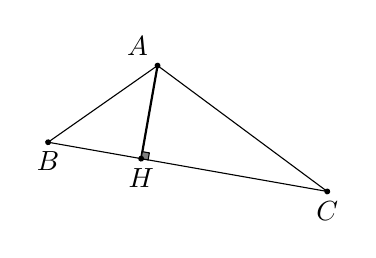
\begin{tikzpicture}[rotate=-10,scale=0.6]
            \coordinate (H) at (0,0);
            \coordinate (A) at (0,2);
            \coordinate (B) at (-2,0);
            \coordinate (C) at (4,0);
            \draw (A) -- (B) -- (C) -- cycle;
            \draw[thick] (A) -- (H);
            \node[above left] at (A) {$A$};
            \node[below] at (B) {$B$};
            \node[below] at (C) {$C$};
            \node[below] at (H) {$H$};
            \draw[fill=gray] (H) rectangle ($(H)+(0.15,0.15)$);
            \draw[fill=black] (A) circle (0.05);
            \draw[fill=black] (B) circle (0.05);
            \draw[fill=black] (C) circle (0.05);
            \draw[fill=black] (H) circle (0.05);
        \end{tikzpicture}\hspace{2cm}
        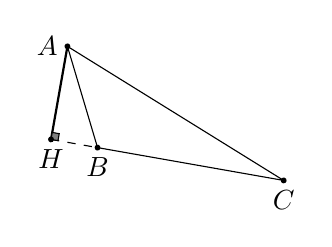
\begin{tikzpicture}[rotate=-10,scale=0.6]
            \coordinate (H) at (0,0);
            \coordinate (A) at (0,2);
            \coordinate (B) at (1,0);
            \coordinate (C) at (5,0);
            \draw (A) -- (B) -- (C) -- cycle;
            \draw[thick] (A) -- (H);
            \draw[dashed] (H) -- (B);
            \node[left] at (A) {$A$};
            \node[below] at (B) {$B$};
            \node[below] at (C) {$C$};
            \node[below] at (H) {$H$};
            \draw[fill=gray] (H) rectangle ($(H)+(0.15,0.15)$);
            \draw[fill=black] (A) circle (0.05);
            \draw[fill=black] (B) circle (0.05);
            \draw[fill=black] (C) circle (0.05);
            \draw[fill=black] (H) circle (0.05);
        \end{tikzpicture}
        \end{center}

        \item Il est capable de dire que dans le losange $ACBD$, ses diagonales permettent de former $4$ triangles rectangles en $E$.

        \begin{center}
        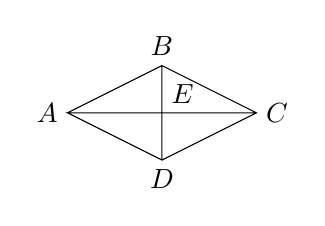
\begin{tikzpicture}[scale=0.6]
            \node[left] at (0,0) {$A$};
            \node[above] at (2,1) {$B$};
            \node[right] at (4,0) {$C$};
            \node[below] at (2,-1) {$D$};
            \node[above right] at (2,0) {$E$};
            \draw (0,0) -- (2,1) -- (4,0) -- (2,-1) -- (0,0) -- (4,0) (2,1) -- (2,-1);
        \end{tikzpicture}
        \end{center}

        \item 
        \begin{minipage}[t]{0.7\textwidth}
            Il sait décomposer une figure complexe telle que celle ci-contre en identifiant les figures simples qui la constituent.
        \end{minipage}\hfill
        \begin{minipage}{0.2\textwidth}
            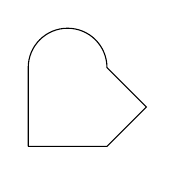
\begin{tikzpicture}[scale=0.5]
                \draw (0,0) -- (0,2) arc (180:0:1) -- (3,1) -- (2,0) -- (0,0);
            \end{tikzpicture}
        \end{minipage}

        \item[] \textit{Dans l’espace}
        \item 
        \begin{minipage}[t]{0.7\textwidth}
            Il est capable de dire que le solide suivant est constitué d’un cylindre surmonté d’un cône de sommet $D$, et que $[DA]$ est la hauteur de ce cône.
        \end{minipage}\hfill
        \begin{minipage}{0.1\textwidth}
            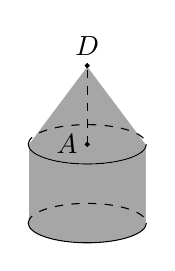
\begin{tikzpicture}[scale=0.5]
                \coordinate (A) at (0,0);
                \coordinate (D) at (0,2);
                \coordinate (O) at ($(A)+(-1.5,0)$);
                \coordinate (P) at ($(A)+(-1.5,-2)$);
    
                \draw[white,fill=gray!70!white] (P) -- (O) arc(180:360:1.5cm and 0.5cm) -- ($(P)+(3,0)$) arc(360:180:1.5cm and 0.5cm) -- (O);
                \draw[white,fill=gray!70!white] (O) arc(180:360:1.5cm and 0.5cm) -- (D) -- (O);
                
                \draw (O) arc(180:360:1.5cm and 0.5cm);
                \draw[dashed] (O) arc(180:0:1.5cm and 0.5cm);
                \draw (P) arc(180:360:1.5cm and 0.5cm);
                \draw[dashed] (P) arc(180:0:1.5cm and 0.5cm);
                
                \draw[dashed] (A) -- (D);
                \draw[fill=black] (A) circle (0.05);
                \draw[fill=black] (D) circle (0.05);
                \node[left] at (A) {$A$};
                \node[above] at (D) {$D$};
            \end{tikzpicture}
        \end{minipage}
    \end{exemplesreussite}

    \souscompetence{Reproduire, représenter, construire}
    \begin{savoireleves}
        \item[] \textit{Dans le plan}
        \item Il représente, reproduit, trace ou construit des figures simples.
        \item Il représente, reproduit, trace ou construit des \textit{figures complexes} (assemblages de figures simples).
        \item Il réalise, complète ou rédige un programme de construction d’une figure plane.\\
        Il réalise une figure plane simple ou une figure composée de figures simples à l’aide d’un logiciel de géométrie dynamique.
        \item[] \textit{Dans l'espace}
        \item Il représente un cube, un pavé droit par un dessin.
        \item Il construit un patron d’un pavé droit.\\
        Il construit une maquette à l’aide de patrons d’un assemblage de solides simples (cube, pavé droit, prisme droit, pyramide) dont les patrons sont donnés pour les prismes et les pyramides.
    \end{savoireleves}

    \clearpage
    \begin{exemplesreussite}
        \item[] \textit{Dans le plan}
        \vspace{-0.7cm}
        
        \item 
        \begin{minipage}[t]{0.65\textwidth}
            Le texte suivant lui étant donnée : \\
            « Trace le triangle $ABC$ isocèle en $B$, sachant que $AB = \qty{6}{\centi\metre}$ et que $AC = \qty{4}{\centi\metre}$. » \\
            Il est capable de faire un dessin à main levée, codé comme ci-contre, avant de construire la figure à l’aide d’une règle et d’un compas.
        \end{minipage}\hspace{0.07\textwidth}
        \begin{minipage}{0.25\textwidth}
            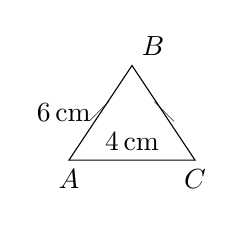
\begin{tikzpicture}[scale=0.4]
                 \coordinate (A) at (0,0);
                 \coordinate (C) at (4,0);
                 \coordinate (B) at (2,3);
                 \draw (A) -- (B) -- (C) -- cycle;
                 \node[rotate=45] at ($(A)!0.5!(B)$) {|};
                 \node[rotate=-45] at ($(C)!0.5!(B)$) {|};
                 \node[below] at (A) {$A$};
                 \node[above right] at (B) {$B$};
                 \node[below] at (C) {$C$};
                 \node[above] at ($(A)!0.5!(C)$) {\qty{4}{\centi\metre}};
                 \node[left] at ($(A)!0.5!(B)$) {\qty{6}{\centi\metre}};
            \end{tikzpicture}
        \end{minipage}

        \item[\CR] Construis un triangle $ABC$ avec $AB = \qty{6.2}{\centi\metre}$, $BC = \qty{2.7}{\centi\metre}$ et $AC = \qty{4.1}{\centi\metre}$.
        \item Le texte suivant lui étant donné : « Trace le rectangle $DEFG$ tel que $DE = 6 cm$ et que $DF = 8 cm$. », il est capable de faire un dessin à main levée, codé comme ci-dessous, et de voir le rectangle comme la juxtaposition de $2$ triangles rectangles identiques pour le construire.

        \begin{center}
        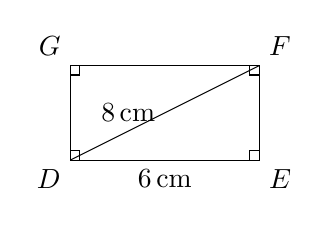
\begin{tikzpicture}[scale=0.4]
            \coordinate (D) at (0,0); 
            \coordinate (E) at (6,0);
            \coordinate (F) at (6,3);
            \coordinate (G) at (0,3);
            \draw (D) -- (E) -- (F) -- (G) -- cycle;
            \node[below left] at (D) {$D$};
            \node[below right] at (E) {$E$};
            \node[above right] at (F) {$F$};
            \node[above left] at (G) {$G$};
            \draw (D) -- (F);
            \node[below] at ($(D)!0.5!(E)$) {\qty{6}{\centi\metre}};
            \node[left] at ($(D)!0.5!(F)$) {\qty{8}{\centi\metre}};
            \draw (D) rectangle ($(D)+(0.3,0.3)$);
            \draw (E) rectangle ($(E)+(-0.3,0.3)$);
            \draw (F) rectangle ($(F)+(-0.3,-0.3)$);
            \draw (G) rectangle ($(G)+(0.3,-0.3)$);
        \end{tikzpicture}
        \end{center}

        \item À partir d’une description écrite, d’un programme de construction, il est capable de faire une représentation à main levée codée et de construire à l’aide des instruments une figure simple.
        \item[\CR] Construis un carré dont les diagonales mesurent \qty{5}{\centi\metre}.
        \item[\CR] Construis un losange $ABCD$ dont les diagonales mesurent \qty{6.4}{\centi\metre} et \qty{3}{\centi\metre}.
        \item Pour construire le carré $ABCD$ dont le côté mesure \qty{8}{\centi\metre}, il est capable de dire ou d’écrire : « Je commence par tracer le segment $[AB]$ mesurant \qty{8}{\centi\metre}, puis la droite perpendiculaire à la droite $(AB)$ passant par $B$, sur cette droite, je place un point $C$ tel que $BC = \qty{8}{\centi\metre}$... »
        \item 
        \begin{minipage}[t]{0.7\textwidth}
            À l’aide d’un logiciel de géométrie dynamique, il est capable de reproduire un dessin comme ci-contre pouvant être agrandi ou réduit en déplaçant un seul point des points initiaux.
        \end{minipage}\hfill
        \begin{minipage}{0.2\textwidth}
            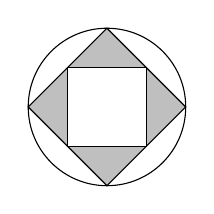
\begin{tikzpicture}
            \tikzmath{\rayon = 1;}
                \coordinate (O) at (0,0);
                \draw (O) circle (\rayon);
                \coordinate (A) at ($(O)+(0,\rayon)$);
                \coordinate (B) at ($(O)+(-\rayon,0)$);
                \coordinate (C) at ($(O)+(0,-\rayon)$);
                \coordinate (D) at ($(O)+(\rayon,0)$);
                \draw[fill=gray!50!white] (A) -- (B) -- (C) -- (D) -- cycle;
                \draw[fill=white] ($(A)!0.5!(B)$) -- ($(B)!0.5!(C)$) -- ($(C)!0.5!(D)$) -- ($(D)!0.5!(A)$) -- cycle;
            \end{tikzpicture}
        \end{minipage}

        \item[] \textit{Dans l'espace} 
        \item Il est capable, sur quadrillage ou sur papier blanc, de représenter un morceau de sucre par un dessin comme ci-dessous.

        \begin{center}
        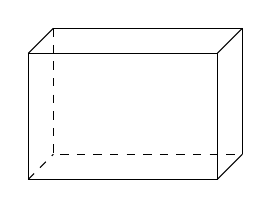
\begin{tikzpicture}[scale=0.8]
            \coordinate (A) at (0,0);
            \coordinate (B) at (3,0);
            \coordinate (C) at (3,2);
            \coordinate (D) at (0,2);
            \coordinate (u) at (0.4,0.4);
            \coordinate (A') at ($(A)+(u)$);
            \coordinate (B') at ($(B)+(u)$);
            \coordinate (C') at ($(C)+(u)$);
            \coordinate (D') at ($(D)+(u)$);
            \draw (A) -- (B) -- (C) -- (D) -- cycle;
            \draw[dashed] (D') -- (A') -- (B');
            \draw (B') -- (C') -- (D');
            \draw[dashed] (A) -- (A');
            \draw (B) -- (B') (C) -- (C') (D) -- (D');
        \end{tikzpicture}
        \end{center}
        
        \item 
        \begin{minipage}[t]{0.8\textwidth}
            Il est capable de produire, un patron d’un pavé dont les dimensions sont données. Par exemple, pour le patron d’un pavé dont les dimensions sont \qty{2}{\centi\metre}, \qty{3}{\centi\metre} et \qty{4}{\centi\metre}, il produit sur quadrillage ou sur papier blanc une figure comme ci-contre.
        \end{minipage}\hfill
        \begin{minipage}{0.1\textwidth}
            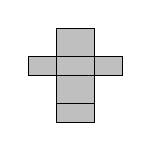
\begin{tikzpicture}[scale=0.12]
                \draw[fill=gray!50!white] (0,0) rectangle (3,2);
                \draw[fill=gray!50!white] (3,0) rectangle (7,2);
                \draw[fill=gray!50!white] (7,0) rectangle (10,2);
                \draw[fill=gray!50!white] (3,2) rectangle (7,5);
                \draw[fill=gray!50!white] (3,0) rectangle (7,-3);
                \draw[fill=gray!50!white] (3,-3) rectangle (7,-5);
            \end{tikzpicture}
        \end{minipage}
        \item Il est capable, par exemple, de produire les patrons des pavés nécessaires pour faire une maquette de podium comme ci-dessous.

        \begin{center}
        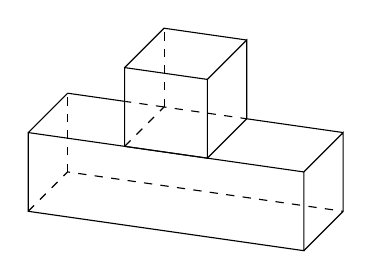
\begin{tikzpicture}[scale=0.5]
            % Vecteur pour la perspective cavalière
            \coordinate (u) at (1,1);

            % Grand pavé droit
            \coordinate (A) at (0,0);
            \coordinate (B) at (7,-1);
            \coordinate (C) at (7,1);
            \coordinate (D) at (0,2);
            \coordinate (A') at ($(A)+(u)$);
            \coordinate (B') at ($(B)+(u)$);
            \coordinate (C') at ($(C)+(u)$);
            \coordinate (D') at ($(D)+(u)$);
            \draw (A) -- (B) --  (C) -- (D) -- cycle;
            \draw (D) -- (D');
            \draw (B) -- (B') -- (C') -- (C);
            \draw[dashed] (A) -- (A') -- (B');
            \draw[dashed] (A') -- (D');

            % Petit cube au dessus
            \coordinate (E) at ($(D)!0.35!(C)$);
            \coordinate (F) at ($(D)!0.65!(C)$);
            \coordinate (G) at ($(F)+(0,2)$);
            \coordinate (H) at ($(E)+(0,2)$);
            \coordinate (E') at ($(E)+(u)$);
            \coordinate (F') at ($(F)+(u)$);
            \coordinate (G') at ($(G)+(u)$);
            \coordinate (H') at ($(H)+(u)$);
            \draw (E) -- (F) -- (G) -- (H) -- cycle;
            \draw (G) -- (G') -- (F') -- (F);
            \draw (G') -- (H') -- (H);
            \draw[dashed] (E) -- (E') -- (F');
            \draw[dashed] (E') -- (H');

            % Reliure des deux
            \draw (C') -- (F');
            \draw[dashed] (E') -- ($(E')!0.4!(D')$);
            \draw ($(E')!0.4!(D')$) -- (D');
        \end{tikzpicture}
        \end{center}
    \end{exemplesreussite}

    \clearpage
    \competence{Reconnaître et utiliser quelques relations géométriques}

    \begin{savoireleves}
        \item[] \textit{\textbf{Alignement, segments}}
        \item Il connaît la définition de l’alignement de $3$ points ainsi que de l’appartenance à une droite et reconnaît ces situations.
        \item Il connaît, reconnaît et sait tracer un segment de droite ainsi que son milieu.
        \item Relations de perpendicularité et de parallélisme
        \item Il connaît les relations entre perpendicularité et parallélisme et sait s’en servir pour raisonner.
        \item Il détermine le plus court chemin entre un point et une droite.
        \item Il connaît et sait estimer la distance entre un point et une droite.
        \item[] \textit{\textbf{Symétrie axiale}}
        \item Il complète une figure par symétrie axiale.
        \item Il construit le symétrique d’un point, d’un segment, d’une droite par rapport à un axe donné et il est capable de verbaliser/expliciter sa méthode de construction.
        \item Il construit la figure symétrique d’une figure donnée par rapport à un axe donné sur papier ou à l’aide d’un logiciel de géométrie dynamique.
        \item Il connaît les propriétés de conservation de la symétrie axiale et il les utilise pour raisonner.
        \item Il connaît, reconnaît et sait coder la définition de la médiatrice d’un segment, ainsi que sa caractérisation.
        \item Il sait se servir de la définition de la médiatrice d’un segment ou de sa caractérisation pour la tracer à l’aide des instruments adéquats.
        \item[] \textit{\textbf{Proportionnalité}}
        \item Il reproduit une figure en respectant une échelle donnée.
    \end{savoireleves}

    \begin{exemplesreussite}
        \item[] \textit{\textbf{Relations de perpendicularité et de parallélisme}}
        \item Dans une situation comme ci-dessous, il trace la droite $(AB)$ pour pouvoir dire quels sont les points alignés avec les points $A$ et $B$.

        \begin{center}
        \begin{tikzpicture}
            \tikzmath{\taille = 0.05;}
            \coordinate (A) at (0,0);
            \coordinate (B) at (5,0.5);
            \coordinate (C) at (7,0.9);
            \coordinate (D) at (8,0.8);
            \coordinate (E) at (9,0.85);
            \coordinate (F) at (10,0.45);
            \coordinate (G) at (11,1.1);
            \coordinate (H) at (-1,-0.1);
            \draw ($(A)!-0.1!(B)$) -- ($(A)!1.1!(B)$);
            \foreach \p in {A,B,C,D,E,F,G,H} {
                \draw[red] ($(\p)+(\taille,\taille)$) -- ($(\p)+(-\taille,-\taille)$);
                \draw[red] ($(\p)+(-\taille,\taille)$) -- ($(\p)+(\taille,-\taille)$);
                \node[red,above right] at (\p) {$\p$};
            }
        \end{tikzpicture}
        \end{center}

        \item Il sait que si $I$ est le milieu du segment $[AB]$ avec $AB = \qty{4}{\centi\metre}$, alors $I$ est le point du segment $[AB]$ tel que $IA = IB = \qty{2}{\centi\metre}$ et il sait le coder.

        \begin{center}
        \begin{tikzpicture}
            \tikzmath{\taille = 0.05;}
            \coordinate (A) at (0,0);
            \coordinate (B) at (3,2);
            \coordinate (I) at ($(A)!0.5!(B)$);
            \draw (A) -- (B);
            \foreach \p in {A,B,I} {
                \draw ($(\p)+(\taille,\taille)$) -- ($(\p)+(-\taille,-\taille)$);
                \draw ($(\p)+(-\taille,\taille)$) -- ($(\p)+(\taille,-\taille)$);
                \node[above left] at (\p) {$\p$};
            }
            \foreach \u/\v in {A/I,B/I} {
                \node[rotate=30] at ($(\u)!0.5!(\v)$) {||};
            }
        \end{tikzpicture}
        \end{center}

        \item Il sait que $2$ droites perpendiculaires à une même droite sont parallèles.
        \item Il sait que si deux droites sont parallèles alors toute perpendiculaire à l’une est perpendiculaire à l’autre.
        \item 
        \begin{minipage}[t]{0.7\textwidth}
            Dans la situation ci-contre, il est capable de dire que les droites $(AC)$ et $(BD)$ étant toutes les deux perpendiculaires à la droite $(AB)$, elles sont parallèles.
        \end{minipage}\hfill
        \begin{minipage}{0.15\textwidth}
            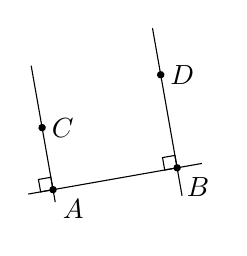
\begin{tikzpicture}[rotate=10,scale=0.8]
                \coordinate (A) at (0,0);
                \coordinate (B) at (2,0); 
                \coordinate (C) at (0,1);
                \coordinate (D) at (2,1.5);
                \draw ($(C)!-1!(A)$) -- ($(C)!1.2!(A)$);
                \draw ($(A)!-0.2!(B)$) -- ($(A)!1.2!(B)$);
                \draw ($(B)!-0.3!(D)$) -- ($(B)!1.5!(D)$);
                \foreach \p/\position in {A/{below right}, B/{below right}, C/right, D/right} {
                    \draw[fill=black] (\p) circle (0.05);
                    \node[\position] at (\p) {$\p$};
                }
                \draw (A) rectangle ($(A)+(-0.2,0.2)$);
                \draw (B) rectangle ($(B)+(-0.2,0.2)$);
            \end{tikzpicture}
        \end{minipage}
        \item Il sait que le plus court chemin d’un point $C$ à une droite $(AB)$ est de suivre la perpendiculaire à $(AB)$ passant par $C$.

        \clearpage
        \item Dans une situation comme ci-dessous, il sait que la distance entre le point $D$ et la droite $(AB)$ est égale à la longueur du segment $[DH]$ où $H$ est le point d’intersection entre la droite $(AB)$ et sa perpendiculaire passant par $D$.

        \begin{center}
        \begin{tikzpicture}[rotate=10]
            \coordinate (A) at (0,0);
            \coordinate (B) at (2,0);
            \coordinate (I) at (2.8,0);
            \coordinate (D) at (2.8,2);
            \draw ($(A)!-0.2!(I)$) -- ($(A)!1.4!(I)$);
            \draw[dashed] ($(I)!-0.3!(D)$) -- ($(I)!1.1!(D)$);
            \draw (I) rectangle ($(I)+(-0.2,0.2)$);
            \foreach \p in {A,B,I,D} {
                \draw[fill=black] (\p) circle (0.05);
                \node[above right] at (\p) {$\p$};
            }
        \end{tikzpicture}
        \end{center}

        \item Il est capable de compléter les deux figures ci-dessous pour que la droite verticale soit un axe de symétrie.

        \begin{center}
        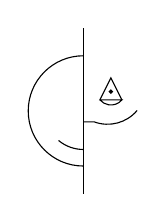
\begin{tikzpicture}[scale=0.7]
            \draw (0,0.5) -- (0,3.5);
            \draw (0,1) arc(270:90:1);
            \draw (0,1.3) arc(270:230:0.7);
            \draw (0,1.8) -- (0.2,1.8) arc (250:320:0.7);
            \draw[fill=black] (0.5,2.35) circle (0.03);
            \draw (0.7,2.2) -- (0.5,2.6) -- (0.3,2.2) -- (0.7,2.2) arc (320:220:0.26);
        \end{tikzpicture}\hspace{1cm}
        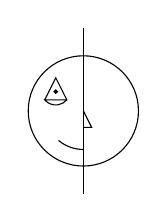
\begin{tikzpicture}[scale=0.7]
            \draw (0,0.5) -- (0,3.5);
            \draw (0,2) circle (1);
            \draw (0,1.3) arc(270:230:0.7);
            \draw[fill=black] (-0.5,2.35) circle (0.03);
            \draw (-0.7,2.2) -- (-0.5,2.6) -- (-0.3,2.2) -- (-0.7,2.2) arc (220:320:0.26);
            \draw (0,2) -- (0.15,1.7) -- (0,1.7);
        \end{tikzpicture}
        \end{center}

        \item Sur papier blanc, il est capable de compléter une figure comme ci-dessous à gauche pour tracer l’image du point $C$ par la symétrie axiale d’axe $(AB)$, et d’expliquer que pour cela il doit tracer la perpendiculaire à la droite $(AB)$ passant par $C$, puis reporter la distance de $C$ à $(AB)$ sur cette perpendiculaire pour obtenir l’image de $C$ (comme sur la figure de droite).

        \begin{center}
        \begin{tikzpicture}[scale=0.8,rotate=-40]
            \coordinate (A) at (0,3);
            \coordinate (B) at (0,0);
            \coordinate (C) at (-2,2);
            \draw (A) -- (B);
            \foreach \p in {A,B,C} {
                \node[left] at (\p) {$\p$};
                \draw[fill=black] (\p) circle (0.05);
            }
            \draw[rotate=40,thick,-latex] (3,1.5) -- (5.4,1.5); 
        \end{tikzpicture}\hspace{1cm}
        \begin{tikzpicture}[scale=0.8,rotate=-40]
            \coordinate (C') at (2,2);
            \draw (A) -- (B);
            \draw[dotted] ($(C)!-0.2!(C')$) -- ($(C)!1.2!(C')$);
            \draw (C) -- (C');
            \foreach \p in {A,B,C,C'} {
                \node[left] at (\p) {$\p$};
                \draw[fill=black] (\p) circle (0.05);
            }
            \draw (0,2) rectangle (-0.2,2.2);
            \node at ($(C)!0.25!(C')$) {||};
            \node at ($(C)!0.75!(C')$) {||};
        \end{tikzpicture}
        \end{center}

        \item Sur une feuille blanche, il est capable de construire le symétrique d’un point, d’un segment, d’une droite ou d’une figure par rapport à un axe donné en utilisant l’équerre et la règle graduée ou le compas et une règle non graduée Exemple : Construire les figures symétriques des figures $CDEFG$, $HIJ$ et du cercle par rapport à la droite $(AB)$.

        \begin{center}
        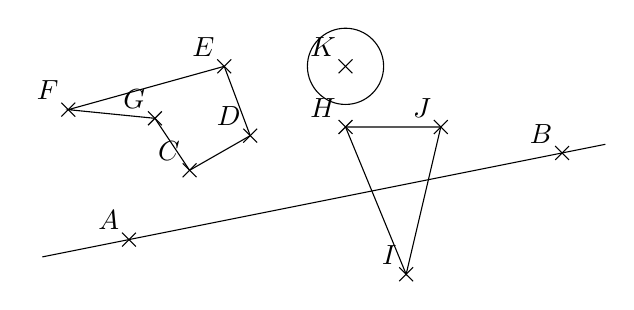
\begin{tikzpicture}[scale=1.1]
            \tikzmath{\taille = 0.08;}
            \coordinate (A) at (0,0);
            \coordinate (B) at (5,1);
            \coordinate (C) at (0.7,0.8);
            \coordinate (D) at (1.4,1.2);
            \coordinate (E) at (1.1,2);
            \coordinate (F) at (-0.7,1.5);
            \coordinate (G) at (0.3,1.4);
            \coordinate (H) at (2.5,1.3);
            \coordinate (I) at (3.2,-0.4);
            \coordinate (J) at (3.6,1.3);
            \coordinate (K) at (2.5,2);

            \foreach \p in {A,B,...,K} {
                \draw ($(\p)+(\taille,\taille)$) -- ($(\p)+(-\taille,-\taille)$);
                \draw ($(\p)+(-\taille,\taille)$) -- ($(\p)+(\taille,-\taille)$);
                \node[above left] at (\p) {$\p$};
            }

            \draw ($(A)!-0.2!(B)$) -- ($(A)!1.1!(B)$);
            \draw (C) -- (D) -- (E) -- (F) -- (G) -- cycle;
            \draw (H) -- (I) -- (J) -- cycle;
            \draw (K) circle (0.44);
        \end{tikzpicture}
        \end{center}

        \item Il est capable compléter une figure comme ci-dessous pour tracer sa symétrique par rapport à la droite.

        \begin{center}
        \begin{tikzpicture}[scale=0.21]
            \draw[gray!20!white] (0,0) grid (15,15);
            \coordinate (A) at (8,5);
            \coordinate (B) at (8,1);
            \draw (1,14) -- (14,1);
            \draw (A) -- (1,9) -- (1,5) arc (180:270:4) -- (B) -- (A);
            \draw (A) -- (5,5) -- (5,1);  
            \draw (1,5) -- (5,5);
            \foreach \p in {A,B} {
                \draw[fill=black] (\p) circle (0.1);
                \node[right] at (\p) {$\p$};
            }
        \end{tikzpicture}
        \end{center}

        Pour tracer l’image de la figure précédente, il est capable de dire la symétrie axiale conservant les longueurs et les mesures angulaires il lui suffit de tracer les images des points $A$ et $B$ puis d’utiliser le quadrillage pour terminer sa construction.
        \item Il sait que la médiatrice d’un segment est la droite perpendiculaire au segment en son milieu.
        \item Il sait que tous les points de la médiatrice d’un segment sont à égale distance des extrémités de ce segment.

        \clearpage
        \item Il sait également que l’ensemble des points équidistants des extrémités d’un segment est sa médiatrice.
        \item Sur des figures comme celle-ci-dessous, il reconnaît la médiatrice du segment $[AB]$.
        \begin{center}
        \begin{tikzpicture}
            \coordinate (A) at (0,0);
            \coordinate (B) at (4,0);
            \draw (A) -- (B);
            \draw (2,-2) -- (2,2);
            \draw (2,0) rectangle (2.2,0.2);
            \node at (1,0) {|};
            \node at (3,0) {|};
            \foreach \p in {A,B} {
                \draw[fill=black] (\p) circle (0.05);
                \node[below] at (\p) {$\p$};
            }
        \end{tikzpicture}\hspace{1cm}
        \begin{tikzpicture}
            \coordinate (A) at (0,0);
            \coordinate (B) at (4,0);
            \coordinate (E) at (2,1);
            \coordinate (F) at (2,-3);
            \draw (A) -- (B);
            \draw (2,-3.3) -- (2,1.3);
            \node[rotate=45] at ($(A)!0.5!(E)$) {|};
            \node[rotate=-45] at ($(B)!0.5!(E)$) {|};
            \node[rotate=-45] at ($(A)!0.5!(F)$) {||};
            \node[rotate=45] at ($(B)!0.5!(F)$) {||};
            \draw[dashed] (A) -- (E) -- (B) -- (F) -- cycle;
            \foreach \p/\ori in {A/left,B/right,E/{above right},F/{below right}} {
                \draw[fill=black] (\p) circle (0.05);
                \node[\ori] at (\p) {$\p$};
            }
        \end{tikzpicture}
        \end{center}

        \item Il utilise son équerre pour tracer la médiatrice d’un segment en s’appuyant sur sa définition.

        \begin{center}
        \begin{tikzpicture}
            \draw (0,0) -- (10,4);
            \draw[latex-latex] (0,-0.2) -- (5,1.8);
            \draw[fill=black] (5,2) circle (0.08);
            \node[below right] at (5,2) {$AB=10$};
            \node[above] at (2.5,1.2) {$\qty{5}{\centi\metre}$};
            \draw[fill=black] (0,0) circle (0.06);
            \draw[fill=black] (10,4) circle (0.06);
            \node[left] at (0,0) {$A$};
            \node[right] at (10,4) {$B$};

            % équerre
            \coordinate (e1) at (5.05,2.1);
            \coordinate (e2) at (8,3.3);
            \coordinate (e3) at (4.25,4.1);
            \definecolor{equerre}{HTML}{B3D1E9}
            \draw[fill=equerre] (e1) -- (e2) -- (e3) -- cycle;
            \coordinate (u) at (-0.4,1);
            \coordinate (v) at (1,0.4);
            \draw[fill=white] ($(e1)+0.4*(v)+0.4*(u)$) -- ($(e2)-1.1*(v)+0.4*(u)$) -- ($(e3)+0.4*(v)-0.5*(u)$) -- cycle;

        \end{tikzpicture}
        \end{center}

        \item Il utilise son compas pour tracer la médiatrice d’un segment en s’appuyant sur sa caractérisation.

        \begin{center}
        \begin{tikzpicture}
            \coordinate (A) at (0,0);
            \coordinate (B) at (4,-1);
            \foreach \p in {A,B} {
                \draw[fill=black] (\p) circle (0.03);
                \node[below] at (\p) {$\p$};
            }
            \draw (A) -- (B);
            \draw ({3*cos(-50)},{3*sin(-50}) arc (-50:-100:3);
            \draw ($(B) + ({3*cos(-120)},{3*sin(-120})$) arc (-120:-160:3);
            \draw ({3*cos(20)},{3*sin(20}) arc (20:50:3);
            \draw ($(B) + ({3*cos(100)},{3*sin(100})$) arc (100:130:3);
        \end{tikzpicture}
        \end{center}

        \item Il est capable d’agrandir les figures suivantes pour que les figures obtenues soient $1,5$ fois plus grandes (les longueurs affichées sont en \unit{\centi\metre}).

        \begin{center}
        \begin{tikzpicture}[scale=0.5]
            \tikzmath{\taille = 0.12;}
            \coordinate (A) at (0,0);
            \coordinate (B) at (4,0);
            \coordinate (C) at (4,3);
            \draw (A) -- (B) -- (C) -- cycle;

            \foreach \p/\ori in {A/left,B/right,C/above} {
                \draw ($(\p)+(0.8*\taille,\taille)$) -- ($(\p)+(-0.8*\taille,-\taille)$);
                \draw ($(\p)+(-0.8*\taille,\taille)$) -- ($(\p)+(0.8*\taille,-\taille)$);
                \node[\ori] at (\p) {$\p$};
            }
            \node[below] at ($(A)!0.5!(B)$) {$4$};
            \node[above left] at ($(A)!0.5!(C)$) {$5$};
            \node[right] at ($(B)!0.5!(C)$) {$3$};
        \end{tikzpicture}\hspace{1cm}
        \begin{tikzpicture}
            \tikzmath{\taille = 0.12;}
            \coordinate (D) at (0,0);
            \coordinate (E) at (0.866,0.5);
            \draw (D) circle (1);
            \foreach \p/\ori in {D/{above left},E/right} {
                \draw ($(\p)+(0.8*\taille,\taille)$) -- ($(\p)+(-0.8*\taille,-\taille)$);
                \draw ($(\p)+(-0.8*\taille,\taille)$) -- ($(\p)+(0.8*\taille,-\taille)$);
                \node[\ori] at (\p) {$\p$};
            }
            \draw (D) -- (E);
        \end{tikzpicture}\hspace{1cm}
        \begin{tikzpicture}[scale=0.3]
            \coordinate (P) at (0,0);
            \coordinate (E) at (8,0);
            \coordinate (L) at (8,7);
            \coordinate (O) at (2.622,6.49);
            \draw (P) -- (E) -- (L) -- (O) -- cycle;
            \node[below] at ($(P)!0.5!(E)$) {\qty{8}{\centi\metre}};
            \node[rotate=-90,above] at ($(L)!0.5!(E)$) {\qty{7}{\centi\metre}};
            \node[rotate=68,above] at ($(P)!0.5!(O)$) {\qty{7}{\centi\metre}};
            \draw ($(P)!0.1!(E)$) arc (0:68:0.8);
            \node at ($(P)+(1.5,0.8)$) {$68$°};
            \foreach \p/\ori in {P/left,E/right,L/{above right},O/{above left}} {
                \node[\ori] at (\p) {$\p$};
            }
        \end{tikzpicture}
        \end{center}
    \end{exemplesreussite}
\end{document}